\documentclass[a4paper,10pt,italian]{article}
\textwidth 460pt
\textheight 700pt
\hoffset -60pt
\voffset -80pt
%\usepackage[latin1]{inputenc}
\usepackage{babel}
\usepackage{graphicx}
\usepackage{textcomp}
\usepackage{amsmath}
\usepackage{amssymb}
\usepackage{epstopdf}
\usepackage[applemac]{inputenc}
\usepackage{color}

%===========================================================================
% SIMBOLI SISTEMA
%===========================================================================
% 1: scritta a sinistra
% 2: scritta dentro il box
% 3: scritta a destra
%===========================================================================

\newcommand{\SISTEMA}[3]
{
	\begin{center}
	\begin{picture}(270,40)
		%box
		\put(100,5){\line(1,0){80}}
		\put(180,5){\line(0,1){30}}
		\put(180,35){\line(-1,0){80}}
		\put(100,35){\line(0,-1){30}}
		%contenuto box
		\put(110,17){#2}
		%frecce
		\put(80,20){\vector(1,0){20}}
		\put(180,20){\vector(1,0){20}}
		%testo sinistra e destra
		\put(40,20){#1}
		\put(210,20){#3}
	\end{picture}
	\end{center}
}

%===========================================================================
% SIMBOLI SISTEMA SERIE
%===========================================================================
% 1: ingresso
% 2: scritta dentro il primo box
% 3: segnale intermedio
% 4: scritta dentro il secondo box
% 5: uscita
%===========================================================================

\newcommand{\SISTEMASERIE}[5]
{
	\begin{center}
	\begin{picture}(300,40)
		%box1
		\put(50,5){\line(1,0){70}}
		\put(120,5){\line(0,1){30}}
		\put(120,35){\line(-1,0){70}}
		\put(50,35){\line(0,-1){30}}
		%box2
		\put(180,5){\line(1,0){70}}
		\put(250,5){\line(0,1){30}}
		\put(250,35){\line(-1,0){70}}
		\put(180,35){\line(0,-1){30}}
		%frecce
		\put(30,20){\vector(1,0){20}}
		\put(120,20){\vector(1,0){60}}
		\put(250,20){\vector(1,0){20}}
		%ingresso
		\put(5,17){#1}
		%testo 1 box
		\put(60,17){#2}
		%segnale intermedio
		\put(140,28){#3}
		%testo 2 box
		\put(190,17){#4}
		%uscita
		\put(280,17){#5}
	\end{picture}
	\end{center}
}

%===========================================================================
% SIMBOLI SISTEMA PARALLELO
%===========================================================================
% 1: ingresso
% 2: scritta dentro il primo box
% 3: segnale intermedio primo box
% 4: scritta dentro il secondo box
% 5: segnale intermedio secondo box
% 6: uscita
%===========================================================================

\newcommand{\SISTEMAPARALLELO}[6]
{
	\begin{center}
	\begin{picture}(260,100)
		%box1
		\put(80,5){\line(1,0){70}}
		\put(150,5){\line(0,1){30}}
		\put(150,35){\line(-1,0){70}}
		\put(80,35){\line(0,-1){30}}
		%box2
		\put(80,45){\line(1,0){70}}
		\put(150,45){\line(0,1){30}}
		\put(150,75){\line(-1,0){70}}
		\put(80,75){\line(0,-1){30}}
		%frecce
			%freccia sopra sinistra
			\put(40,60){\vector(1,0){40}}
			%freccia sotto sinistra
			\put(50,20){\vector(1,0){30}}
			%linea sinistra verso il basso
			\put(50,60){\line(0,-1){40}}
			%freccia uscita box1
			\put(150,60){\vector(1,0){56}}
			%linea uscita box2
			\put(150,20){\line(1,0){60}}
			%freccia destra verso l'alto
			\put(210,20){\vector(0,1){36}}
			%freccia uscita
			\put(214,60){\vector(1,0){20}}
		%simbolo somma
		\put(210,60){\circle{8}}
		%ingresso
		\put(10,57){#1}
		%testo 1 box
		\put(90,57){#2}
		%segnale intermedio 1
		\put(160,70){#3}
		%testo 2 box
		\put(90,17){#4}
		%segnale intermedio 2
		\put(160,30){#5}
		%uscita
		\put(240,57){#6}
	\end{picture}
	\end{center}
}


%===========================================================================
% SIMBOLI NUOVI
%===========================================================================

\newcommand{\sinc}[0]{\mbox{sinc}}
\newcommand{\tri}[0]{\mbox{tri}}
\newcommand{\rect}[0]{\mbox{rect}}
\newcommand{\DTFT}[0]{\mbox{DTFT}}
\newcommand{\DFT}[0]{\mbox{DFT}}
\newcommand{\convcirc}[0]{\otimes}
\newcommand{\trasfz}[0]{\stackrel{\mbox{Z}}{\longleftrightarrow}}


\DeclareGraphicsRule{.tif}{png}{.png}{`convert #1 `dirname #1`/`basename #1 .tif`.png}

%\DeclareGraphicsRule{.png}{bmp}{.bb}{}

\title{Elaborazione Numerica dei Segnali A}
\author{Proudly provided by PicciMario\\\emph{http://piccimario.wordpress.com}}
%\date{}

\begin{document}

\maketitle

This work is licensed under the Creative Commons Attribution-Noncommercial-Share Alike 2.5 Italy License. To view a copy of this license, visit http://creativecommons.org/licenses/by-nc-sa/2.5/it/.

\tableofcontents

\newpage

\begin{quote}
\underline{Segnale}: supporto fisico dell'informazione \\\\
$\Downarrow$ modellizzazione matematica \\\\
\underline{Funzioni} \\
monodimensionali (1 variabile indipendente)\\
bidimensionali (2 variabili indipendenti).
\end{quote}

\section{Classificazione dei segnali}
\begin{itemize}
	\item $x(t)$ segnale analogico
	\item $x(kT)$ segnale a tempo discreto (campionato)
	\item $x_q(t)$ segnale quantizzato
	\item $x[n]$ segnale numerico (a tempo discreto, quantizzato)
\end{itemize}

\section{Segnale numerico}

$$ \vec{x} \in \Re \mbox{ (o C)} \qquad : \qquad \vec{x} = \{ x[n], -\infty \leq n \leq +\infty, n \in Z\} $$

\subsection{Rappresentazione dei segnali numerici}
\begin{itemize}
	\item Rappresentazione grafica
		\begin{figure}[htbp] %  figure placement: here, top, bottom, or page
		   \centering
		   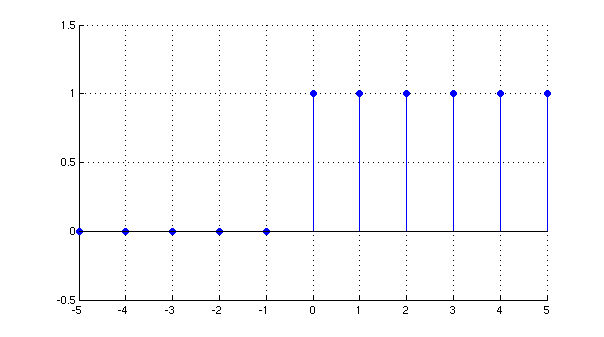
\includegraphics[width=8cm]{img/gradino.png} 
		\end{figure}
	\item Rappresentazione sequenziale
		\begin{align*}
		x[n] = \{ 1,2,&1,1,2,3,4 \}\\
		&\uparrow \mbox{\emph{rappresenta la posizione dell'elemento di indice 0.}}
		\end{align*}
	\item Rappresentazione tabulare
	\item Rappresentazione funzionale\\
		$$x[n] = a^n\sin(2\pi f_0 n)$$
\end{itemize}

\subsection{Supporto/durata di un segnale numerico}
Il supporto \'e il pi\'u piccolo insieme di indici n al di fuori dei quali il segnale assume il valore $x[n]=0$ in modo costante.\\
La durata \'e il numero di indici del supporto.

\subsection{Dinamica di un segnale numerico}
$D = max_n \{ x[n] \} - min_n \{ x[n] \}  $\\\\
NB: in valori intermedi agli indici (sempre interi) il valore di x \'e NON DEFINITO, non 0.

\subsection{Energia/Potenza di un segnale}
\begin{itemize}
	\item Energia di un segnale a tempo discreto\\
		$$ W_x = \sum_{n=-\infty}^{+\infty} \mid x[n] \mid ^2$$\\
		se $W_x < \infty \Rightarrow$ \underline{segnale di energia} (segnale a energia finita)
	\item Potenza media di un segnale a tempo discreto\\
		$$ P_x = \lim_{N\to +\infty} \frac{1}{2N+1} \sum_{n=-N}^{N} \mid x[n] \mid^2$$\\
		se $P_x < \infty$ e $P_x \neq 0 \Rightarrow$ \underline{segnale di potenza} (segnale a potenza media finita non nulla)
\end{itemize}

\subsection{Sequenza periodica}
Una sequenza $x[n]$ si dice periodica se $\exists N$ tale che:
$$ x[n] = x[n+N] \qquad \forall n \in Z$$
$M = min\{N_i\}$ si dice \underline{periodo fondamentale} del segnale a tempo discreto.\\\\
I segnali periodici a tempo discreto di periodo fondamentale M sono a potenza media finita non nulla.\\\\
Potenza media di un segnale periodico a tempo discreto $x[n]$ con periodo M:
$$ P_x = \frac{1}{M} \sum_{n_0}^{n_0+M-1} \mid x[n] \mid^2$$

\subsection{Classificazione temporale}
\begin{itemize}
	\item sequenze causali $x[n]=0 \quad \forall n<0$
	\item sequenze anticausali $x[n]=0 \quad \forall n \geq 0$
	\item sequenza non causali $\quad \exists \quad n_1 \geq 0\quad n_2 < 0 \quad : \quad x[n_1]\neq 0\quad x[n_2]\neq 0$
	\item sequenza "right-sided": supporto limitato solo a sinistra.
	\item sequenza "left-sided": supporto limitato solo a destra.
	\item sequenza limitata ($W_x \mbox{ sempre } < \infty$)
	\item sequenza illimitata.
\end{itemize}

\subsection{Simmetrie}
\begin{itemize}
	\item segnale pari: $ x[n]=x[-n] $
	\item segnale dispari: $ x[n] = -x[-n] $
	\item sequenza a simmetria pari rispetto a $n_0$
	\begin{itemize}
		\item $n_0 \in Z$ (simmetria pari rispetto al campione $n_0$)
			$$ x[n_0+n] = x[n_0-n] $$
		\item $n_0 \not\in Z$, ma $2n_0 \in Z $ (simmetria pari rispetto al mezzo campione $n_0$)
			$$ x\Bigr[n_0+n+\frac{1}{2}\Bigr] = x\Bigr[n_0-n-\frac{1}{2}\Bigr] $$
	\end{itemize}
	\item sequenza a simmetria dispari rispetto a $n_0$ ($x[n_0] = 0 !!!$)
	\begin{itemize}
		\item $n_0 \in Z$ (simmetria dispari rispetto al campione $n_0$)
			$$ x[n_0+n] = -x[n_0-n] $$
		\item $n_0 \not\in Z$, ma $2n_0 \in Z $ (simmetria dispari rispetto al mezzo campione $n_0$)
			$$ x\Bigr[n_0+n+\frac{1}{2}\Bigr] = -x\Bigr[n_0-n-\frac{1}{2}\Bigr] $$
	\end{itemize}
	\item sequenza a simmetria coniugata pari: $ x[n]=x^*[-n] $ (parte reale pari, immaginaria dispari)
	\item sequenza a simmetria coniugata dispari: $ x[n] = -x^*[-n] $ (parte reale dispari, immaginaria pari)
\end{itemize}

\subsection{Operazioni elementari}
\begin{itemize}
	\item Somma di sequenze
		$$ y[n] = x_1[n] + x_2[n] $$
	\item Prodotto di sequenze
		$$ y[n] = x_1[n] \cdot x_2[n] $$
		NB: somme e prodotti di segnali periodici producono sempre un segnale periodico, con periodo pari al MCM dei periodi dei segnali di partenza.
		Questo perch\'e i periodi sono per forza in rapporto razionale tra di loro.
	\item Divisione di sequenze
		$$ y[n] = x_1[n] / x_2[n] \quad,\quad x_2[n]\neq 0 \quad \forall n $$
	\item Moltiplicazione per una costante
		$$ y[n] = c \cdot x[n] $$
	\item Traslazione
		$$ y[n] = x[n-n_0] $$
		\begin{itemize}
			\item $n_0>0$ traslazione verso destra
			\item $n_0<0$ traslazione verso sinistra
		\end{itemize}
	\item Ribaltamento rispetto a $n=0$
		$$ y[n] = x[-n] $$
	\item Decimazione numerica di un fattore M (compressione)
		$$ y[n] = x[M\cdot n] $$
		Vengono eliminati $M-1$ campioni ogni $M$, a partire $n=0$.
	\item Interpolazione numerica (espansione)
		\begin{align*}
		y[n] \quad &= \quad x[n/L] \quad \mbox{se } n=kL, k \in Z\\
		&= \quad 0 \quad \mbox{altrimenti}
		\end{align*}
		Vengono inseriti $L-1$ campioni di valore nullo tra ciascun campione, a partire da $n=0$.

		\begin{figure}[htp]
		\centering
		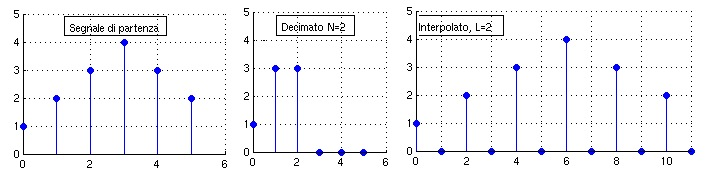
\includegraphics[width=15cm]{img/operazioni.jpg}
		\caption{decimazione e interpolazione, ordine 2}
		\end{figure}

	\item Scomposizione in parte pari e dispari
		\begin{align*}
		x[n] \quad &= \quad x_{sp}[n]+x_{sd}[n]\\\\
		x_{sp}[n_0+n] \quad &= \quad \frac{x[n_0+n]+x[n_0-n]}{2} \\
		x_{sd}[n_0+n] \quad &= \quad \frac{x[n_0+n]-x[n_0-n]}{2} \\
		\end{align*}
		Quindi, per sequenze causali si ha che:
		\begin{align*}
		x_p[n] &= \frac12 x[n]&\mbox{per }n>0\\
			&= x[0]&\mbox{per }n=0\\
		x_d[n] &= \frac12x[n]&\mbox{per } n>0\\
			&= 0&\mbox{per } n=0
		\end{align*}
	
	\item Scomposizione di sequenze complesse in parte coniugata pari e coniugata dispari:
		$$x_{cp}=\frac{x[n]+x^*[-n]}2\qquad x_{cd}=\frac{x[n]-x^*[-n]}2$$

\end{itemize}

%SEGNALI

\newpage

\section{Sequenze elementari}

\subsection{Segnale impulso unitario}
\begin{align*}
\delta[n] = & \quad 1 \quad \mbox{se n=0}\\
& \quad 0 \quad \mbox{altrove}
\end{align*}
\begin{figure}[htp]
\centering
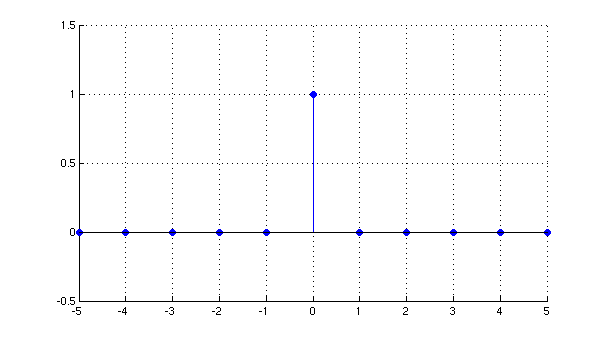
\includegraphics[height=5cm]{img/impulso.png}
\caption{Impulso unitario}
\end{figure}
$\delta[n]$ \'e una sequenza causale. \'E molto diverso da $\delta(t)$, in quanto ha area 1, non $\infty$.\\
Pu\'o essere usato per formare qualunque altro segnale:
$$ x[n] = \sum_{m=-\infty}^{+\infty} x[m]\cdot \delta[n-m] \quad \forall x[n]$$


\subsection{Segnale gradino discreto}
\begin{align*}
\varepsilon[n] = & \quad 1 \quad \mbox{ se } n \geq 0\\
& \quad 0 \quad \mbox{altrove}
\end{align*}
\begin{figure}[htp]
\centering
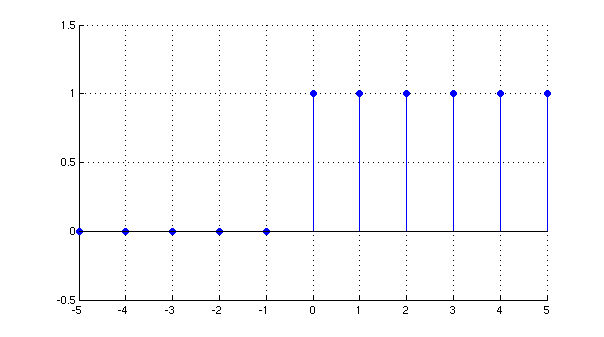
\includegraphics[height=5cm]{img/gradino.png}
\caption{Gradino discreto}
\end{figure}
$\varepsilon[n]$ \'e diverso dal gradino continuo, poich\'e in $n=0$ vale 1, non 0.5.\\
$$ \varepsilon[n] = \sum_{m=0}^{\infty} \delta[n-m] $$
$$ \delta[n] =  \varepsilon[n] - \varepsilon[n-1]$$
\begin{align*}
P_\varepsilon = & \lim_{N\to\infty} \frac{1}{2N+1} \sum_{n=-N}^{+N} \mid \varepsilon[n] \mid ^2\\
= & \lim_{N\to\infty} \frac{1}{2N+1} \sum_{n=0}^{N} 1^2 = \frac{1}{2}
\end{align*}

\subsection{Segnale rettangolo}
\begin{align*}
rect_N[n] = & \quad 1 \quad n \in \{0,1,...,N-1\} \\
= & \quad 0 \quad \mbox{altrimenti}
\end{align*}
\begin{figure}[htp]
\centering
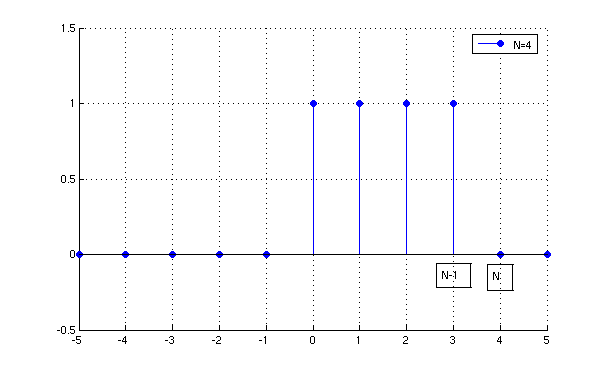
\includegraphics[height=5cm]{img/rect.png}
\caption{Rettangolo discreto}
\end{figure}

$$rect_N[n] = \varepsilon[n] - \varepsilon[n-N]$$
$$ W_x = \sum_{n=-\infty}^{+\infty} \mid rect_N[n] \mid ^2 = \sum_{n=0}^{N-1}1^2 = N$$

\subsection{Sequenza esponenziale reale e causale}
$$ x[n] = a^n\cdot \varepsilon[n] $$
\begin{figure}[htp]
\centering
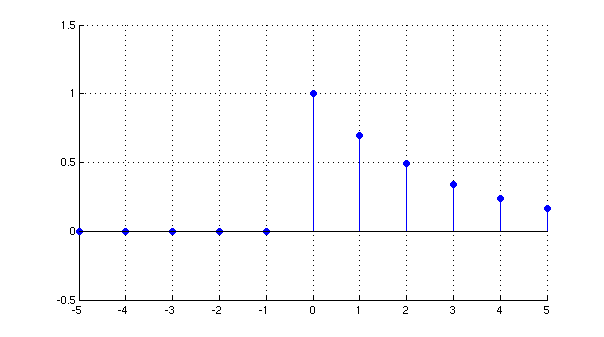
\includegraphics[height=5cm]{img/esponenziale.png}
\caption{Esponenziale $0<a<1$}
\end{figure}

$$W_{a^n\varepsilon[n]}=\sum_{n=0}^{+\infty}(a^2)^n=\frac{1}{1-a^2}$$

\newpage

\subsection{Sequenza sinusoidale di periodo N}
$$ x[n] = A\cdot sin\Bigr(2\pi \frac{n-n_0}{N}\Bigr) $$

\begin{figure}[htp]
\centering
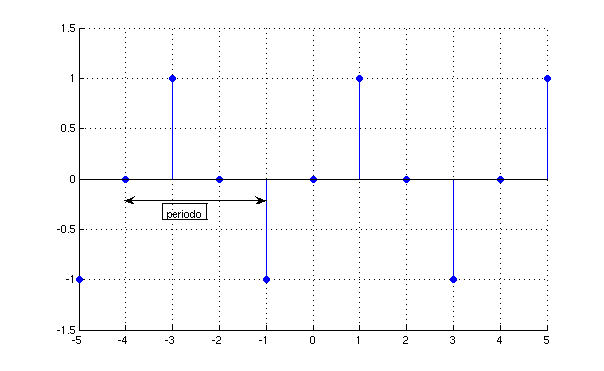
\includegraphics[height=5cm]{img/sin1.png}
\caption{sinusoide, N=4}
\end{figure}
\begin{figure}[htp]
\centering
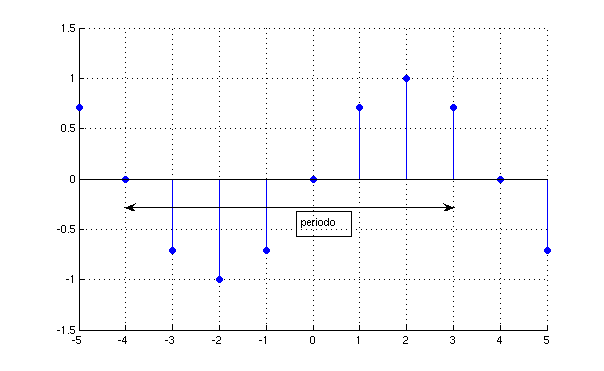
\includegraphics[height=5cm]{img/sin2.png}
\caption{sinusoide, N=8}
\end{figure}

Se $N$ non � intero, il periodo � il pi� piccolo intero multiplo di N. Ad esempio, una sinusoide $x[n]=sin\Bigr(2\pi\frac{3}{4}n\Bigr)$, quindi con frequenza $f_0=\frac34$ ($N=\frac43$) in realt� ha un periodo di 4 (il pi� piccolo multiplo intero di $\frac43$), come se avesse une frequenza $\frac14$. Questo � legato alla periodicit� della \DTFT.

\subsection{Sequenza esponenziale complessa}
\begin{align*}
x[n] \quad = & \quad A \cdot exp(j \cdot 2\pi \cdot f_0 \cdot n) \\
= & \quad A \cdot cos(2\pi \cdot f_0 \cdot n) + j \cdot A \cdot sin(2\pi \cdot f_0 \cdot n)
\end{align*}

%GENERAZIONE DI SEQUENZE DETERMINISTICHE

\section{Generazione di sequenze deterministiche}
\begin{itemize}
\item Campionamento di segnali analogici:
\begin{align*}
\mbox{segnale analogico }x(t)\\
&\Downarrow \quad campionamento\\
\mbox{segnale campionato }x(kT)\\
&\Downarrow \quad quantizzazione\\
&\Downarrow \quad indicizzazione\\
\mbox{Segnale numerico }x[n]
\end{align*}

\item Espressione analitica
$$ x[n]=A\cdot sin\Bigr(2\pi\cdot \frac{n-n_0}{N}\Bigr) $$

\item Equazione alle differenze:\\
Sono equazioni ricorsive corredate da condizioni iniziali. Es:
\begin{align*}
x[n] \quad &= \quad a\cdot x[n-1]\\
x[0] \quad &= \quad 1\\
&\Downarrow\\
x[0] \quad &= \quad 1\\
x[1] \quad &= \quad a\\
x[2] \quad &= \quad a^2\\
\vdots\\
x[n] \quad &= \quad a^n\cdot \varepsilon[n]
\end{align*}

\end{itemize}

\paragraph{Esempio: generazione di sinusoidi a tempo discreto}
\begin{align*}
\sin(\alpha + \beta) \quad &= \quad \sin \alpha \cos \beta + \cos\alpha  \sin\beta \\
\cos(\alpha + \beta) \quad &= \quad \cos\alpha \cos\beta - \sin\alpha \sin\beta 
\end{align*}
ponendo $\alpha = n\beta$
\begin{align*}
\sin((n+1)\beta) \quad &= \quad \sin(n\beta)\cos\beta + \sin\beta\cos(n\beta)\\
\cos((n+1)\beta) \quad &= \quad \cos(n\beta)\cos\beta - \sin(n\beta)\sin\beta
\end{align*}
$x[n] \quad = \quad \sin(n\beta)$\\
$y[n] \quad = \quad \cos(n\beta)$
\begin{align*}
x[n+1] \quad &= \quad x[n]\cos\beta + y[n]\sin\beta\\
y[n+1] \quad &= \quad y[n]\cos\beta - x[n]\sin\beta
\end{align*}
Condizioni iniziali:
\begin{align*}
x[0] \quad &= \quad 0\\
y[0] \quad &= \quad 1
\end{align*}
$\Longrightarrow \quad $ Si ricava $\sin(n\beta)$ e $\cos(n\beta)$

%PROCESSI STOCASTICI

\newpage

\section{Processi Casuali}

Una \underline{sequenza casuale} � una realizzazione di un processo stocastico a tempo discreto.
\\\\
Un \underline{processo stocastico} � una famiglia di sequenze in uno spazio di campioni $\Omega$.
\begin{align*}
	X[n,s)\qquad X:&z\times\Omega\to R\\
			&(n,s)\to X[n,s)
\end{align*}

\begin{figure}[htbp] %  figure placement: here, top, bottom, or page
   \centering
   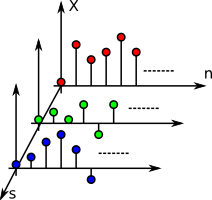
\includegraphics[width=2in]{img/realizzazioni.png} 
   \caption{Processo stocastico}
\end{figure}

Se adesso fisso un tempo $n$, al variare di $s$ osservo una serie di valori casuali, ovvero una variabile casuale $X[n_0]$, caratterizzata da una funzione di distribuzione $F_{x_0}(\alpha)$ e da una pdf (\emph{probability density function}) $f_{x_0}(\alpha)$.

\begin{figure}[htbp] %  figure placement: here, top, bottom, or page
   \centering
   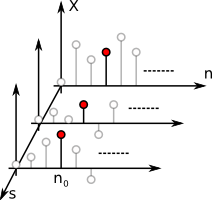
\includegraphics[width=2in]{img/realizzazioni2.png} 
   \caption{Variabile Casuale}
\end{figure}

$F_{X_0}(\alpha)$ rappresenta la probabilit� (da 0 a 1) che la variabile casuale $X_0$ assuma un valore minore o uguale ad $\alpha$.
$$F_{X_0}(\alpha)=p\Bigr(X[n_0,s)\leq\alpha\Bigr)$$
$f_{X_0}(\alpha)$ � la derivata rispetto ad $\alpha$ della funzione di probabilit�.
$$f_{X_0}(\alpha)=\frac{d F_{X_0}}{d \alpha}$$
\\
Dallo schema \ref{fig-fxa} si capisce come la probabilit� che una variabile casuale assuma un certo intervallo di valori � proprio data dall'integrale della sua $f_{X_0}(\alpha)$ sull'intervallo stesso:
$$p(\alpha\leq X_0\leq\alpha+d\alpha)=f_{X_0}(\alpha)\cdot d\alpha$$

\begin{figure}[htbp] %  figure placement: here, top, bottom, or page
   \centering
   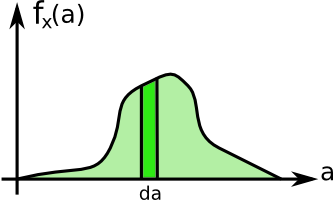
\includegraphics[width=2in]{img/fxa.png} 
   \caption{Probabilit� che la variabile assuma un valore interno a $da$}
   \label{fig-fxa}
\end{figure}

Non basta per� conoscere la pdf di una distribuzione in tutti i possibili valori di $n_0$ per definirla completamente, poich� potrebbe esistere anche una dipendenza tra i valori assunti dalla distribuzione in istanti diversi. \'E necessario andare a studiare la \underline{funzione di distribuzione congiunta}, 
$$F_{X_0, X_1,\dots,X_{K-1}}(\alpha_0,\dots,\alpha_{K-1},n_0,\dots,n_{K-1}) =$$
$$=p\Bigr( X_0\leq\alpha_0, \dots, X_{K-1}\leq\alpha_{K-1} \Bigr)$$
o equivalentemente la \underline{pdf congiunta}.
$$f_{X_0, X_1,\dots,X_{K-1}}(\alpha_0,\dots,\alpha_{K-1},n_0,\dots,n_{K-1}) =$$
$$=\frac{d^KF_{X_0,\dots,X_{K-1}} (\alpha_0,\dots,\alpha_{K-1}, n_0, \dots, n_{K-1}  )}{d\alpha_0,\dots, d\alpha_{K-1}}$$
\\
{\bf Ipotesi di ergodicit�}: supponendo che una distribuzione sia ergodica, � possibile affermare che l'insieme dei valori di una realizzazione si comporta come una variabile casuale $X$ con la stessa pdf rispetto a una qualsiasi delle variavili casuali che possono essere estratte dalla distribuzione stessa fissando un determinato istante $n$.
%\subsection{Valore Atteso}
%Corrisponde alla media di insieme, ovvero alla media pesata di tutte le realizzazioni possibili di una variabile casuale.
%$$ E[X[n]] = \int_{\Re} x_n \cdot f_{X[n]} (x_n) \, dx_n = \mu _n $$ 
%
%\subsection{Autocorrelazione}
%L'autocorrelazione del processo \'e la correlazione tra le variabili casuali $X[n_1]$ e $X[n_2]$
%$$ R_X[n_1,n_2] = E[X[n_1]\cdot X[n_2]] $$
%ovvero:
%$$ \int \int_{\Re^2} x_1 \cdot x_2 \cdot f_{X[n_1],X[n_2]}(x_1,x_2)\,dx_1\,dx_2 $$
%
%\subsection{Stima Campionaria}
%Valore atteso
%$$ E[X(t)] \cong \hat m = \frac{1}{N} \sum_{k=1..N} X(t, s_K) \quad \mbox{con N grande} $$
%Autocorrelazione
%$$ R_X(t_1,t_2) \cong \frac{1}{N} \sum_{k=1..N} X(t_1,s_K).X(t_2,s_k) \quad \mbox{con N grande} $$
%
%\subsection{Stazionariet\'a in senso lato}
%Un processo stocastico in generale si definisce \emph{stazionario} quando le sue caratteristiche 
%statistiche non variano al variare del tempo.\\
%Un processo stocastico in particolare si dice \emph{stazionario in senso lato} (per statistiche del $2^o$ ordine) quando \\ \\
%1) Il valore medio del processo rimane costante nel tempo
%$$ E[X[n]] = \mu _X = costante $$ 
%2) L'autocorrelazione dipende non pi\'u dagli istanti di tempo in cui viene calcolata bens\'i dalla loro distanza.
%\begin{align*}
%R_X(n_1,n_2) &= R_X(n_1+\alpha,\,n_2+\alpha) \quad &\mbox{$\forall$ $\alpha$ costante}\\ 
%&= E[X[n]\cdot X[n+\tau]] \\
%&= R_X[\tau] \quad &\mbox{con $\tau$ = $n_2-n_1$}
%\end{align*}
%
%\subsection{Ergodicit\'a in senso lato}
%Un processo stocastico in generale si definisce \emph{ergodico} quando \'e possibile risalire alle sue 
%caratteristiche statistiche studiando una singola realizzazione.\\
%Un processo stocastico stazionario in particolare si dice \emph{ergodico in senso lato} quando: \\ \\
%1) Il valor medio del processo \'e uguale al valor medio di ogni singola realizzazione.
%$$ E[X[n]] = \lim_{N\to+\infty} \frac{1}{2N+1} \sum_{n=-N}^{N} x[n] = \mu _X $$
%2) L'autocorrelazione del processo \'e uguale all'autocorrelazione di ogni singola realizzazione.
%$$ R_X(\tau) = \lim_{N\to\infty} \frac{1}{2N+1} \sum_{n=-N}^{N} x[n]\cdot x[n+\tau]  $$
\\\\
{\bf L'istogramma} \'e un'approssimante di $f_X(x)$ ottenuto da una serie finita di realizzazioni del processo casuale.
Per realizzare un istogramma, si parte dalla dinamica di $x$ (supponiamo compresa tra A e B) e la si divide in 
un numero C di canali. Poi si comincia a estrarre realizzazioni del processo casuale e le si inserisce nel
canale corrispondente sull'istogramma. Con un numero di realizzazioni $\to\infty$, l'istogramma andr\'a ad 
approssimare la funzione densit\'a.

\begin{figure}[htp]
\centering
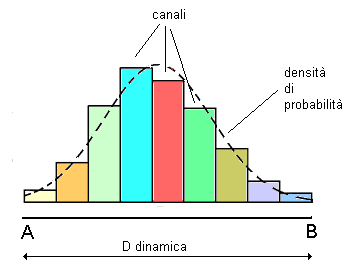
\includegraphics[height=5cm]{img/istogrammi.png}
\caption{istogramma}
\end{figure}

\noindent Quindi, supponendo:
\begin{itemize}
\item N campioni
\item C canali ($l=0...C-1$)
\item $\Delta = \frac{B-A}{C}$
\end{itemize}
La funzione istogramma varr\'a (l-esimo canale):
$$ I_{x,N,C}[l] = \frac{1}{N} \sum_{n=0}^{N-1} \delta \Bigr[ int \Bigr( \frac{X[n]-(l-1)\Delta - B}{\Delta} \Bigr) \Bigr]$$
per N grande $>>$ C grande si ha che:
$$I_{x,N,C}[l]\cong p(\min(x)+(l-1)\Delta\, <X\leq\, \min(x)+l\Delta)\cong f_X\Bigr(\min(x)+(l-1)\Delta+\frac\Delta2\Bigr)\cdot\Delta$$
(per $\Delta$ molto piccolo)

\newpage

\section{Generazione di sequenze pseudo casuali}

\subsection{Generazione di sequenze pseudo casuali con pdf uniforme}
\begin{itemize}
\item sequenze periodiche di periodo N (N molto grande!).
\item limitatamente a un periodo, hanno un andamento che appare casuale.
\end{itemize}

\subsubsection{Prima tecnica: radice primitiva di un numero primo}
$$ X[n+1] = (A\cdot X[n])\,mod\,P \quad A,P \in N^*\quad \mbox{(naturali escluso lo 0)}$$
\begin{itemize}
\item P \'e un numero primo (grande)
\item A \'e una radice primitiva di P, cio\'e\\
$ \forall n \in N^*\quad n<P\quad \exists j \in N^* \quad :\quad n=A^j\,mod\,P $
\end{itemize}
Genera una sequenza periodica di periodo P; ogni numero compreso in $\{ 1,\dots ,P-1 \}$ compare una sola volta all'interno del periodo. In sintesi:
$$ X[n] \in \{ 1,\dots,P \}$$
$$\not\exists (i,j) \mbox{ tale che } X[i]=X[j]\quad i,j\in\{ 0,\dots,P-2 \}$$
abbiamo bisogno di una condizione iniziale 
$$X[0]\in\{ 1,\dots,P-1 \}$$
Per ottenere, normalizzando rispetto a P:
$$ Y[n]=\frac{X[n]}{P} \mbox{ sequenza numerica uniformemente distribuita su } \Bigr[ \frac1p,1+\frac1p\Bigr]\cong[0,1] $$
Esempio:
\begin{itemize}
	\item $P=2^{35}-31$
	\item $A=5^5$
	\item $X[0]=12345$
\end{itemize}

\subsubsection{Seconda tecnica (ricorsiva)}
$$ X[n+1] = (X[n]+X[n-n_0]) \, mod \, 1 $$
\begin{itemize}
\item $n_0 \in N^*$ dev'essere grande (ordine di P)
\item necessit\'a di $n_0+1$ condizioni iniziali su $[0,1]$
\end{itemize}
Genera una sequenza periodica di periodo $n_0$ di valori distribuiti in modo uniforme su $[0,1]$.\\\\
Esempio:
\begin{align*}
n_0 &= 2 \\
X[0] &= 0.32 \\
X[-1] &= 0.19 \\
X[-2] &= 0.47 \\
&\Downarrow \\
X[1] = (X[0]+X[-2])\,mod\,1 &= (0.32+0.47)\,mod\,1 = 0.79 \\
X[2] = (X[1]+X[-1])\,mod\,1 &= (0.79+0.19)\,mod\,1 = 0.98 \\
&\vdots
\end{align*}

\subsubsection{Terza tecnica: algoritmo di Blum Blum Shab}
$$X[n+1]=X^2[n]\,mod\,M$$
M � il prodotto di due numeri primi $P$ e $Q$ grandi, congruenti a $3\,mod\,4$ e tali che $MCD(\Phi(P-1),\Phi(Q-1))$ sia il pi� piccolo possibile. $\Phi$ � la funzione di Eulero, ovvero il numero di numeri primi inferiori all'argomento dato.
\\\\
Realizza una sequenza casuale distribuita uniformemente su $[1,M-1]$, che normalizzata per $M$ diventa una distribuzione uniforme su $[0,1]$.

\subsection{Generazione di sequenze pseudo casuali con altre distribuzioni}
Se abbiamo $x[n]$ che assume valori casuali con pdf uniforme su $[0,1]$
\begin{align*}
f_X(\alpha) \quad &= \quad 1 \quad \mbox{ su } [0,1] \\
&= \quad 0 \quad \mbox{ altrove}
\end{align*}
come si fa a generare una sequenza $Y[n]$ con $f_Y(\beta)$ desiderata?
\SISTEMA{$X, f_X(\alpha)$}{$g(\cdot)$}{$Y=g(X), f_Y(\beta)$}
\begin{itemize}
\item \underline{Step 1}: $ F_Y(\beta)=\int_{-\infty}^{\beta}f_Y(\beta')\,d\beta' $
\item \underline{Step 2:} affermo che $ g(\cdot) = F_Y^{-1}(\cdot) $
\end{itemize}
Dimostrazione:\\
suppongo $g(.)$ invertibile, con inversa $g^{-1}(.)$ (che NON \'e $1/g$!!!)
\begin{align*}
F_Y(\beta) \quad &= \quad p\{ Y \leq \beta \} =\\
&= \quad p\{ g(X)\leq\beta \} = \\
&= \quad p\{ X \leq g^{-1}(\beta) \} =\\
&= \quad F_X(g^{-1}(\beta)) = \\
&= \quad g^{-1}(\beta) \mbox{ poich\'e X ha pdf uniforme.} \\
\\
&\Rightarrow\quad g(\cdot)=F_Y^{-1}(\cdot)
\end{align*}

\subsection{Relazione che lega le pdf delle ampiezze}
\SISTEMA{$X, f_X(\alpha)$}{$g(\cdot)$}{$Y=g(X), f_Y(\beta)$}
$$ f_Y(\beta) = \frac{f_X(\alpha)}{\mid g'(\alpha) \mid _{\alpha = g^{-1}(\beta)} } = \sum_{\alpha=g^{-1}(\beta)}\frac{f_x(\alpha)}{|g'(\alpha)|}$$
(somma per tutti i possibili valori di $\alpha$, potrebbe essercene anche uno solo)

\paragraph{Esempio}: sia $X[n]$ sequenza casuale con pdf uniforme su $[0,1]$. Affermo che 
$$ Y[n] = \sqrt{2\sigma^2\,\ln\frac{1}{X[n]}} $$
Poi calcolo $g^{-1}(\cdot)$:
\begin{align*}
Y^2[n] &= 2\sigma^2\,\ln\frac{1}{X[n]}\\
\ln\frac{1}{X[n]} &= \frac{Y^2[n]}{2\sigma^2}\\
X[n]&= \exp \Bigr( -\frac{Y^2[n]}{2\sigma^2} \Bigr)
\end{align*}
$$\Downarrow$$
\begin{align*}
f_Y(\beta) &= \frac{\beta}{\sigma^2}\,\exp\Bigr( -\frac{\beta^2}{2\sigma^2} \Bigr) \qquad \mbox{ per } \beta>0\\
&= 0 \qquad \mbox{ altrimenti}
\end{align*}
(che \'e una distribuzione di Raleigh)\\\\
Altro esempio: sempre partendo da $X[n]$ con pdf uniforme su $[0,1]$ voglio ottenere:
\begin{align*}
f_Y(\beta) &= \frac{\beta}{2} \qquad 0\leq \beta \leq 2\\
&= 0 \quad \mbox{altrimenti}
\end{align*}
calcolo:
\begin{align*}
F_X(\beta) &= \int_{-\infty}^{\beta} f_Y(\beta')\,d\beta'=\\
&= \int_{0}^{\beta}\frac{\beta'}{2}\, d\beta' = \frac{\beta^2}{4}
\end{align*}
Quindi:
\begin{align*}
F_Y(\beta) &= 0 \qquad \beta<0\\
&= \frac{\beta^2}{4} \qquad 0 \leq \beta \leq 2\\
&= 1 \qquad \beta>2
\end{align*}
Di conseguenza, sapendo che $g(\cdot)=F_Y^{-1}(\cdot)$,
$$ X = \frac{Y^2}{4} \quad \Rightarrow \quad Y = 2\sqrt{\cdot} $$
Quindi 
$$g(\cdot) = 2\sqrt{\cdot}$$

\subsection{Generazione di sequenze pseudo casuali pseudo gaussiane}
Si genera una sequenza $X[n]$ uniforme su $[0,1]$, e si calcola:
$$ Y[n] = \sqrt{2\sigma^2\,\ln\frac{1}{X[n]}} \mbox{ (pdf di Raleigh)}$$
Si generano le due sequenze $Z[n]$ e $W[n]$
\begin{align*}
Z[n]&= Y[n]\cdot\cos(2\pi X[n+1])\\
W[n]&= Y[n]\cdot\sin(2\pi X[n+1])
\end{align*}
che risultano essere gaussiane marginalmente e in modo congiunto, a media nulla e varianza $\sigma^2$.\\
La densit\'a di probabilit\'a congiunta vale:
$$ f_{ZW}(z,w) = \sum_i\frac{f_{XY}(x_i,y_i)}{\mid J(x_i,y_i) \mid} $$
dove $(x_i,y_i)$ sono soluzioni di 
\begin{align*}
Z&=g(x,y)\\
W&=h(x,y)
\end{align*}
Altro metodo: posso generare una sequenza $X[n]$ con pdf gaussiana sfruttando il teorema del limite centrale, il quale afferma che
prendendo $n$ variabili casuali (indipendenti) con pdf qualsiasi e costruendone la variabile casuale somma, per $n\to\infty$ la somma
stessa tende ad assumere un andamento gaussiano.
\begin{align*}
X &= X_1+X_2+\dots+X_n\\
\eta &= \eta_1+\eta_2+\dots+\eta_n\\
\sigma^2 &= \sigma_1^2+\sigma_2^2+\dots+\sigma^2_n
\end{align*}
$$ \lim_{n\to\infty} X = G\Bigr( \frac{x-\eta}{\sigma} \Bigr) \mbox{ (gaussiana con media $\eta$ e varianza $\sigma$)}$$

\section{Convoluzione di segnali}

\subsection{Convoluzione lineare}
Per segnali a energia finita.
$$ Z[n] = X[n] * Y[n] = \sum_{m=-\infty}^{+\infty}X[m]\cdot Y[n-m]$$
Passi per l'esecuzione:
\begin{itemize}
	\item cambio gli indici $n\rightarrow m$
	\item prendo $X[m]$ e lo tengo fisso
	\item prendo $Y[m]$ e lo ribalto, ottenendo $Y[-m]$
	\item traslo $Y[-m]$ di n punti ($n>0$ implica spostamento verso destra)
	\item svolgo il prodotto delle due sequenze
	\item faccio la somma dei campioni della sequenza ottenuta. Questo \'e il valore di $Z[n]$
\end{itemize}

\subsection{Propriet\'a}
\begin{itemize}
	\item Commutativa: 
		$$ X[n]*Y[n]=Y[n]*X[n] $$
		Dimostrazione:
		$$ \sum_{m=-\infty}^{\infty}X[m]Y[n-m] \stackrel{n-m=m'}{=} \sum_{m'=+\infty}^{-\infty}Y[m']X[n-m']=Y[n]*X[n]$$
	\item Distributiva rispetto alla somma:
		$$ X[n]*(Y[n]+Z[n])=X[n]*Y[n]+X[n]*Z[n] $$
		Dimostrazione:
		$$ \sum_{m=-\infty}^{\infty}X[m](Y[n-m]+Z[n-m]) = \sum_{m=-\infty}^{\infty} X[m]Y[n-m] + \sum_{m=-\infty}^{\infty} X[m]Z[n-m] $$
	\item Associativa:
		$$ X[n]*Y[n]*Z[n]=(X[n]*Y[n])*Z[n] $$
	\item Altre:
		\begin{itemize}
			\item se $X[n]$ \'e causale ma $Y[n]$ no:
				$$ X[n]*Y[n]=\sum_{m=0}^{\infty}X[m]Y[n-m]=\sum_{m=-\infty}^{0}Y[m]X[n-m] $$
			\item se entrambi sono causali:
				$$ X[n]*Y[n]=\sum_{m=0}^{n}X[m]Y[n-m]=\sum_{m=0}^{n}Y[m]X[n-m]$$
			\item se $X[n]$ \'e a durata limitata, con supporto $S=\{ n_0,\dots,n_0+N-1 \}$
				$$ X[n]*Y[n]=\sum_{m=n_0}^{n_0+N-1}X[m]Y[n-m]$$
		\end{itemize}
\end{itemize}

\subsection{Supporto del risultato di convoluzione}
Se $X[n]$ ha supporto $\{ n_{0X}, n_{0X}+1,\dots,n_{0X}+N_X-1 \}$ \\
e $Y[n]$ ha supporto $\{ n_{0Y}, n_{0Y}+1,\dots,n_{0Y}+N_Y-1 \}$ \\
allora $Z[n]=X[n]*Y[n]$ ha supporto al pi\'u 
$$ \{ n_{0X}+n_{0Y},\dots, n_{0X}+N_X-1+n_{0Y}+N_Y-1  \} $$
Quindi durata = $N_X+N_Y-1$

\subsection{Convoluzione di sequenze complesse}
\begin{align*}
	X[n] &= X_R[n]+j\cdot X_I[n]\\
	Y[n] &= Y_R[n]+j\cdot Y_I[n]
\end{align*}
\begin{align*}
	X[n]*Y[n] &= (X_R[n]+jX_I[n])\cdot(Y_R[n]+jY_I[n]) =\\\\
	&= X_R[n]*Y_R[n]-X_I[n]*Y_I[n]+j(X_I[n]*Y_R[n]+X_R[n]*Y_I)[n]
\end{align*}

\subsection{Convoluzione normalizzata}
$X[n]$, $Y[n]$ sequenze a potenza media finita non nulla.
$$ X[n]\stackrel{-}{*}Y[n]=\lim_{N\to \infty} \frac{1}{2N+1} \sum_{m=-N}^{N} X[n]Y[n-m]$$

\subsection{Convoluzione circolare}
$X[n]$, $Y[n]$ periodiche di periodo $M_X$ e $M_Y$
$$ X[n]\otimes_MY[n] = \frac{1}{M}\sum_{m=n_0}^{n_0+M-1}X[m]Y[n-m]\qquad \forall n_0 \in Z $$
con $M = m.c.m.(M_X,M_Y)$\\\\
Interpretazione grafica:
\begin{itemize}
\item disegnare il cerchio
\item dividere in M punti ($M=m.c.m.(M_X,M_Y)$)
\item disegnare $X[m]$
\item disegnare $Y[m]$
\item ribaltare $Y[m]$ attorno a un campione qualsiasi
\item spostare $Y[m]$ di un numero di "scatti" pari a $n$
\item eseguire il prodotto
\item sommare i campioni
\item eventualmente normalizzare a $\frac{1}{N}$
\item si \'e ottenuto il valore di $(X \stackrel{-}{\otimes} Y )[n]$
\end{itemize}

\subsection{Complessit\'a del calcolo diretto della convoluzione}
Supponiamo di avere $X[n]$ e $Y[n]$, di durata rispettivamente $N_X$ e $N_Y$, con $N_Y<N_X$.
\begin{itemize}

\item Convoluzione lineare
\begin{align*}
\mbox{Num. prodotti } P&= 1+2+\dots+(N_Y-1) &\mbox{"ingresso segnale"}\\
&+ (N_Y-1)+(N_Y-1)+\dots &N_X-N_Y+1 \mbox{ volte}\\
&+ (N_Y-1)+\dots+2+1 &\mbox{uscita segnale}\\\\
&= N_Y(N_X-N_Y+1)+N_Y(N_Y-1)\\
&= N_X\cdot N_Y\\\\
\mbox{Num. somme } S&= 0+1+2+\dots+(N_Y-2) &\mbox{ingresso segnale}\\
&+N_Y+N_Y+\dots &(N_X-N_Y-1) \mbox{ volte}\\
&+(N_Y-2)+\dots+2+1+0 &\mbox{uscita segnale}\\\\
&=(N_Y-1)(N_Y-N_X-1)+(N_Y-1)(N_Y-2) \\
&= (N_X-1)(N_Y-1)
\end{align*}
\item Convoluzione circolare
\begin{align*}
P &= M^2 \\
S &= M(M-1)
\end{align*}
M: numero traslazioni, M-1: addizioni per periodo
\end{itemize}

\section{CrossCorrelazione di sequenze}
Date le sequenze $X[n]$ e $Y[n]$, la crosscorrelazione \'e un indice di somiglianza tra
$X[n]$ e $Y_m[n]$, dove con $Y_m[n]$ si indica la versione di $Y[n]$ traslata di $m$ campioni.
$$ \varphi_{XY}[m]\quad = \quad \sum_{m=-\infty}^{+\infty}X^*[n]\cdot Y[m+n]$$
che \'e il prodotto scalare tra segnali $<X,Y_m^*>$\\
Operativamente, la crosscorrelazione si svolge come la convoluzione, solo che non c'\'e alcun
ribaltamento di $Y[n]$. Inoltre:
$$ \varphi_{XY}[m]\quad=\quad X^*[-m]*Y[m] $$
La crosscorrelazione NON \'e commutativa, NON \'e associativa e NON \'e causale per sequenze causali.

\subsection{Differenze tra convoluzione e crosscorrelazione}
\begin{center}
\begin{tabular}{c|c}
Convoluzione lineare & Crosscorrelazione\\
\hline
\\$X[n]$, $Y[n]$ causali $\Rightarrow$ $Z[n]$ causale & $X[n]$, $Y[n]$ causali $\Rightarrow$ $Z[n]$ NON causale\\\\
$X[n]$ durata $N_X$, $Y[n]$ durata $N_Y$,\\ $Z[n]$ durata $N_X+N_Y-1$ & uguale\\\\
$P=N_X\cdot N_Y$ & uguale\\\\
Supporto&Supporto\\
$\{n_{0X}+n_{0Y}$,\dots,$n_{0X}+N_X-1+n_{0Y}+N_Y-1\}$ & $\{n_{0Y}-n_{0X}-N_X-1$,\dots,$n_{0Y}+N_Y-1-n_{0X}\}$
\end{tabular}
\end{center}

\subsection{Crosscorrelazione normalizzata}
$X[n]$, $Y[n]$ a potenza media finita non nulla.
$$ \stackrel{-}{\varphi}_{XY}[m]\quad=\quad\lim_{N\to +\infty} \frac{1}{2N+1} \sum_{n=-N}^{N} X^*[n]Y[n+m]\quad=\quad X^*[-m]\stackrel{-}{*}Y[m]$$
$P=N_X+N_Y$

\subsection{Crosscorrelazione circolare}
$X[n]$, $Y[n]$ periodiche di periodo $M_X$, $M_Y$
$$ \stackrel{o}{\varphi}_{XY}[m]\quad=\quad\frac{1}{M}\sum_{m=n_0}^{n_0+M-1}X^*[n]Y[n+m]\quad=\quad X^*[m] \otimes_M Y[m] $$
con $M=m.c.m.(M_X,M_Y)$\\\\
$P=M^2$

\subsection{Crosscorrelazione di sequenze complesse}
\begin{align*}
X[n]&=X_R[n]+j\cdot X_I[n]\\
Y[n]&=Y_R[n]+j\cdot Y_I[n]
\end{align*}
\begin{align*}
\varphi_{XY}[m] \quad &= \quad (X_R+jX_I)^*[-m]*(Y_R)+jY_I)[m] \\
&= \quad \varphi_{X_RY_R}[m]-\varphi_{X_IY_I}[m]+j(\varphi_{X_RY_I}[m]+\varphi_{X_IY_R}[m])
\end{align*}

\subsection{Autocorrelazione}
Se $Y[n]=X[n]$ si parla di autocorrelazione:
$$ \varphi_X[m]\quad = \quad \sum_{n=-\infty}^{+\infty} X^*[n]Y[n+m] $$
in particolare:
$$ \varphi_X[0]\quad=\quad \mid\mid X \mid\mid^2\quad = \quad W_X $$

\subsection{Crosscorrelazione e distanza}
$$ d^2(X,Y) \quad = \quad \mid\mid X-Y \mid\mid ^2 \quad = \quad \sum_{n=-\infty}^{+\infty} \mid X[n]-Y[n] \mid^2 $$
$$ d^2(X,Y_m) \quad=\quad \mid\mid X \mid\mid^2 + \mid\mid Y \mid\mid ^2 - 2\Re\{ \varphi_{XY}[m] \} $$
NB: distanza massima $\Rightarrow$ correlazione minima

\subsection{Hermitianit\'a}
$$ \varphi_{XY}[m]\quad=\quad \varphi_{YX}^*[-m] $$
(deriva dall'hermitianit\'a del prodotto scalare)\\
Per quanto riguarda l'autocorrelazione:
$$ \varphi_X[m] \quad = \quad \varphi_X[-m] $$
inoltre, se $X[m]$ \'e reale, $\varphi_X[m]=\varphi_X[-m]$ e l'autocorrelazione \'e pari.

\subsection{Disuguaglianza di Schwartz}
$$ \mid \varphi_{XY}[m]\mid \quad \leq \quad \mid\mid X \mid\mid\cdot\mid\mid Y \mid\mid $$
Se $X[m]=Y[m]$:
$$ \mid \varphi_{XY}[m] \mid \quad \leq \quad \mid\mid X \mid\mid^2 \quad = \quad P_X \mbox{ oppure } W_X$$
Inoltre:
\begin{align*}
\mid \varphi_{XY}[0]\mid^2 \quad \leq \quad \varphi_X[0]&\cdot\varphi_Y[0]\\
\downarrow \, & \,  \downarrow \\
\mid\mid X \mid\mid^2 & \mid\mid Y \mid\mid^2
\end{align*}
NB: per segnali di energia il massimo di $\varphi_X[m]$ \'e in 0, dove vale $\varphi_X[0]=\mid\mid X \mid\mid ^2 = W_X$\\\\
NB2: per segnali periodici di periodo $M_X$, $\varphi_X$ \'e periodica con massimi in $k\cdot M_X$ dove vale $\mid\mid X \mid\mid^2 = P_X$

\section{Elaborazione di sequenze numeriche}
\SISTEMA{$x[n]$}{$S[\cdot]$}{$y[n]$}
$S[\cdot]$ \'e detto \emph{Sistema a tempo discreto}: $y[n]=S[x[n]]$
%\\\\Esempi:
%\begin{enumerate}
%\item Quadratore (non lineare, causale, senza memoria, tempo-invariante, stabile)
%$$ y[n]=x^2[n] $$
%\item Mediatore (lineare, causale, con memoria, tempo-invariante, stabile)
%$$ y_2[n]=\frac{x[n]+x[n-1]}{2} $$
%\item Filtro mediano (di durata 5) (non lineare, non causale, con memoria, tempo-invariante, stabile)\\
%Si prende una finestra larga 5 centrata sul valore di $n$ che si vuole calcolare, si ordina la sequenza
%ricavata in ordine crescente e si prende il valore mediano (in posizione 3 della finestra).\\
%Utile per eliminare i disturbi di tipo impulsivo.
%\end{enumerate}

\subsection{Classificazione dei sistemi}

\subsubsection{Linearit\'a del sistema}
$S[\cdot]$ \'e detto lineare se e solo se:
\begin{enumerate}
	\item $\forall x_1[n],x_2[n]$ sequenze:
		$$ S[x_1[n]+x_2[n]] = S[x_1[n]]+S[x_2[n]] \qquad \mbox{Principio di sovrapposizione} $$
	\item $\forall \alpha \in C$
		$$ S[\alpha\cdot x_1[n]] = \alpha\cdot S[x_1[n]] \qquad \mbox{Condizione di Omogeneit\'a}$$
\end{enumerate}
$\Rightarrow\forall \alpha_1,\alpha_2 \in C$, $x_1[n],x_2[n]$ sequenze qualsiasi, si ha che:
$$ S[\alpha_1\cdot x_1[n] + \alpha_2\cdot x_2[n]] = \alpha_1 \cdot S[x_1[n]]+\alpha_2 \cdot S[x_2[n]] $$

\subsubsection{Causalit\'a del sistema}
$S[\cdot]$ \'e causale se $y[n]$ dipende solamente dei valori dell'ingresso $x[n]$ in istanti precedenti
o al pi\'u il presente ($\forall x[n]$).\\\\
$S[\cdot]$ \'e anticausale se $y[n]$ dipende solamente da valori dell'ingresso nel futuro (anche il 
presente \'e escluso).\\\\
In tutti gli altri casi il sistema \'e non causale.

\subsubsection{Memoria del sistema}
$S[\cdot]$ \'e detto senza memoria se $y[n]$ dipende dell'ingresso solo nell'istante $n$.\\\\
$S[\cdot]$ \'e detto con memoria se $y[n]$ dipende dell'ingresso in istanti anche diversi dall'instante corrente.
\begin{align*}
	\mbox{Nota: con memoria} &\Rightarrow \mbox{o anticausale, o causale, o non causale} \\
	\mbox{senza memoria} &\Rightarrow \mbox{causale}
\end{align*}

\subsubsection{Invarianza alla traslazione}
$S[\cdot]$ \'e invariante alla traslazione se $\forall x[n]$ sequenza in ingresso, $n_0 \in Z$
$$ y[n] \stackrel{\triangle}{=} S[x[n]] $$
allora:
$$ S[x[n-n_0]] = y[n-n_0] $$

\subsubsection{Stabilit\'a del sistema}
$S[\cdot]$ \'e stabile se $\forall$ sequenza $x[n]$ tale che 
$$\mid x[n] \mid < \infty \quad \forall n$$
allora 
$$\mid S[x[n]] \mid < \infty$$

\subsection{Sistemi Lineari Tempo-invarianti (LTI)}
Sono i sistemi lineari e invarianti alla traslazione.
\begin{align*}
	&x[n] = x[n]*\delta[n] = \sum_{m=-\infty}^{\infty} x[m]\cdot \delta[n-m] \\
	\mbox{per linearit\'a }&\Downarrow\\
	&S[x[n]] = S\Bigr[ \sum_{m=-\infty}^{\infty} x[m]\cdot\delta[n-m] \Bigr] = \sum_{m=-\infty}^{\infty}x[m]\cdot S[\delta[n-m]]\\
	\mbox{per tempo-invarianza }&\Downarrow \\
	&\mbox{se } h[n]\stackrel{\triangle}{=} S[\delta[n]] \qquad \Rightarrow \qquad S[\delta[n-m]]=h[n-m]\\
	&\mbox{quindi } S[x[n]]=\sum_{m=-\infty}^{\infty}x[m]\cdot h[n-m] = x[n]*h[n]
\end{align*}
Si ha una quindi:
\SISTEMA{$x[n]$}{LTI}{$y[n]=x[n]*h[n]$}
\begin{center}
dove $h[n]=S[\delta[n]]$
\end{center}
Ci sono 2 situazioni possibili:
\begin{enumerate}
	\item FIR (finite impulse response): \\\\
	$h[n]$ ha durata finita $N_h$: $h[n]=0$ se $n\not\in \{ n_0,n_0+1,\dots ,n_0+N_h-1 \}$
	\begin{align*}
		y[n] &= \sum_{m=n_0}^{n_0+N_h-1} x[n-m]\cdot h[m]\\
		&= x[n-n_0]h[n_0]+x[n-n_0+1]h[n_0+1]+\dots+x[n-n_0+N_h-1]h[n_0+N_h-1]
	\end{align*}
	$n_0 \geq 0$ $\Rightarrow$ causale\\
	$n_0 < 0$ e $n_0+N_h-1 \geq 0$ $\Rightarrow$ non causale\\
	$n_0+N_h-1 < 0$ $\Rightarrow$ anticausale

	\item IIR (infinite impulse response): \\\\
	$h[n]$ ha durata infinita
	\begin{itemize}
		\item se $h[n]$ right-sided:
		$$ y[n]=\sum_{m=n_0}^{\infty}x[n-m]h[m]=\sum_{m=-\infty}^{n_0}x[m]h[n-m] $$
		causale se $n_0 \geq 0$, altrimenti non causale
		\item se $h[n]$ left-sided:
		$$ y[n]=\sum_{m=-\infty}^{n_0}x[n-m]h[m]=\sum_{m=n_0}^{\infty}x[m]h[n-m] $$
		anticausale se $n<0$, altrimenti non causale
		\item se $h[n]$ two-sided:
		$$ y[n]=\sum_{m=-\infty}^{\infty} x[n-m]h[m] $$
		non causale
	\end{itemize}
\end{enumerate}

\subsubsection{Causalit\'a dei sistemi LTI}
Un sistema LTI \'e causale se e solo se $h[n]$ \'e una sequenza causale ($h[n]=0 \quad \forall \quad n<0$). Infatti:
$$ y[n]=\sum_{m=-\infty}^{\infty}h[m]x[n-m]=\sum_{m=0}^{\infty}h[m]x[n-m] $$

\subsubsection{Stabilit\'a dei sistemi LTI}
Un sistema LTI \'e stabile se e solo se $h[n]$ \'e assolutamente sommabile:
$$ \sum_{m=-\infty}^{\infty}\mid h[m] \mid < \infty$$
\'E una condizione sufficiente, in quanto si pu\'o dimostrare che se $\mid x[n] \mid < \infty \quad \forall n$ allora
$y[n]$, che \'e pari alla sommatoria di convoluzione tra $x[n]$ e $h[n]$, \'e $<0 \quad \forall n$ (se \'e 
rispettata la condizione del teorema sopra).\\
Inoltre \'e anche una condizione necessaria, in quanto se non \'e rispettata l'ipotesi \'e sempre possibile trovare
un $x[n]$ che, pur non divergendo, faccia divergere $y[n]$.

\subsubsection{Esempi}
\begin{enumerate}
	\item Ritardatore puro
	$$y[n]=x[n-n_0]$$
	$$h[n]=\delta[n-n_0]$$
	Se $n_0 \geq 0$ il sistema � causale, se $n_0 < 0$ il sistema � anticausale (anticipatore). \\
	Il suo inverso � il sistema: $h_I[n]=\delta[n+n_0]$.\\
	\'E un sistema FIR (quindi stabile).

	\item Mediatore su $N$ campioni
	$$ y_M[n] = \frac{1}{N} \sum_{m=n_1}^{n_1+N-1} x[n-m] $$
	$$h_M[n]=\frac1N\mbox{rect}_N[n-n_1]$$
	\'E un sistema FIR (quindi stabile), causale (se $n_1\geq0$).
	
	\item Accumulatore
	$$ y[n]=\sum_{m=-\infty}^{n} x[m] = \sum_{m=n}^{\infty}x[n-m] $$
	$$ h[n]=\varepsilon[n] $$
	\'E un sistema IIR causale instabile.

	\item Differenziatore numerico
	$$y[n]=x[n]-x[n-1]$$
	$$h[n]=\delta[n]-\delta[n-1]$$
	\'E un sistema FIR, stabile, causale.

	\item $h[n]=a^n\cdot \varepsilon[n] \quad$ con $\mid a \mid < 1$\\\\
	sistema LTI IIR right-sided causale stabile\\\\
	stabile poich\'e $\sum_{n=-\infty}^{\infty} a^n = \lim_{n\to N} \sum_{n=0}^{N} a^n =$ serie geometrica $= \frac{1}{1-a}$
\end{enumerate}
Un sistema FIR non causale o anticausale pu\'o essere sempre 
reso causale con la messa in cascata di un opportuno ritardo.

\subsubsection{Cascata di sistemi LTI}
(per sistemi a tempo discreto)
\SISTEMASERIE{$x[n]$}{$h_1[n]$ LTI}{$y_1[n]$}{$h_2[n]$ LTI}{$y_2[n]$}
\begin{align*}
	y_1[n]&=x[n]*h_1[n]\\\\
	y_2[n]&=y_1[n]*h_2[n]=(x[n]*h_1[n])*h_2[n]=\\
	&\Downarrow \mbox{ per associativit\'a}\\
	&=(h_1[n]*h_2[n])*x[n]
\end{align*}
Il che \'e equivalente a dire:
\SISTEMA{$x[n]$}{$h_1[n]*h_2[n]$}{$y_2[n]$}

\subsubsection{Parallelo di sistemi LTI}
\SISTEMAPARALLELO{$x[n]$}{$h_1[n]$}{$y_1[n]$}{$h_2[n]$}{$y_2[n]$}{$y[n]$}
\begin{align*}
	y[n] &= y_1[n]+y_2[n] = (x[n]*h_1[n])+(x[n]*h_2[n])=\\
	&= x[n]*(h_1[n]+h_2[n])
\end{align*}
Il che \'e equivalente a dire:
\SISTEMA{$x[n]$}{$h_1[n]+h_2[n]$}{$y[n]$}

\subsubsection{Inverso di un sistema LTI}
Un sistema LTI con risposta all'impulso $h[n]$ ammette un sistema LTI inverso con risposta all'impulso
$h_I[n]$ se \'e possibile trovare un $h_I[n]$ tale che $h[n]*h_I[n]=\delta[n]$
\SISTEMASERIE{$x[n]$}{$h[n]$}{$y[n]$}{$h_I[n]$}{$x[n]$}
$$ (h[n]*h_I[n])*x[n]= x[n] $$
$$ \Leftrightarrow h[n]*h_I[n]=\delta[n] $$
\\\
\paragraph{Esempio} Accumulatore 
$$ h[n]=\varepsilon[n] $$
il suo inverso \'e il derivatore
$$ h_I[n]=\delta[n]-\delta[n-i] $$
Dimostrazione:
$$ h[n]*h_I[n]=\varepsilon[n]*(\delta[n]-\delta[n-1])=\varepsilon[n]-\varepsilon[n-i]=\delta[n] $$

\subsection{Equazioni alle differenze}
Equazioni ricorsive tra ingresso e uscita nel tempo.
$$ \sum_{k=0}^{N} a_k\cdot y[n-k] = \sum_{l=0}^{M} b_l\cdot x[n-l] $$
Alcuni sistemi LTI possono essere descritti equivalentemente (alla convoluzione) mediante equazioni
alle differenze con condizioni iniziali al riposo.
\begin{enumerate}
	\item \'e sempre vero per i FIR
	\begin{align*}
		y[n] &= \sum_{l=0}^{M}h[l] \cdot [n-l]\\
		&= \sum_{l=0}^{M}\frac{b_l}{a_0}\cdot x[n-l]
	\end{align*}
	(in questo esempio non \'e stata introdotta la ricorsione rispetto all'uscita negli istanti precedenti)\\\\
	Nota: un'espressione equivalente pu\'o essere ottenuta utilizzando valori dell'uscita in istanti precedenti:\\\\
	\emph{Esempio}: mediatore su N campioni (causale)
	\begin{align*}
		y[n] &= \frac{1}{N}\sum_{m=0}^{N-1}x[n-m] &\mbox{senza ricorsione rispetto alle uscite}\\
		&= \frac{N\cdot y[n-1]+x[n]-x[n-N]}{N} &\mbox{con ricorsione}
	\end{align*}
	
	\item \'e vero per alcuni IIR\\\\
	\emph{Esempio}:
	\SISTEMA{$x[n]$}{differenziatore}{$y[n]=x[n]-x[n-1]$}
	\SISTEMA{$y[n]$}{accumulatore}{$x[n]$}
	\begin{align*}
		y[n] &= x[n]*\varepsilon[n]\\
		&= \sum_{m=-\infty}^{\infty} x[m] &\mbox{senza ricorsione}\\
		&= y[n-1]+x[n] &\mbox{con ricorsione}
	\end{align*}
\end{enumerate}

\subsection{Soluzioni di equazioni lineari alle differenze}
Equazione alle differenze:
$$ \sum_{n=0}^{N} a_k\cdot y[n-h] = \sum_{l=0}^{M}b_l\cdot x[n-l] $$
nel caso causale:
\begin{align*}
	y[n] &= \sum_{k=1}^{N} \Bigr( -\frac{a_k}{a_0} \Bigr)y[n-k] + \sum_{l=0}^{M}\Bigr( \frac{b_l}{a_0} \Bigr)x[n-l]\\
	&= \sum_{k=1}^{N}a'_k\cdot y[n-h]+\sum_{l=0}^{M}b'_l \cdot x[n-l] & a'_k=-\frac{a_k}{a_0}\quad b'_l=\frac{b_l}{a_0}
\end{align*}
\begin{enumerate}
	\item Risoluzioni in modo ricorsivo con N condizioni iniziali 
	per $y[-1],y[-2],\dots ,y[-N]$ per il calcolo di $n=0,1,\dots ,\infty$ 

	\item Risoluzione in modo analitico
	$$ y[n]=y_p[n]+y_o[n] $$
	\begin{itemize}
		\item $y_p[n]$: soluzione omogenea, ovvero la soluzione dell'equazione senza ingressi
		$$ \sum_{k=0}^{N}a_K\cdot y[n-k]=0 $$
		sapendo che, in generale:
		$$ y_o[n]=\sum_{m=0}^{N}\alpha_m z_m^n $$
		unendo le due equazioni precedenti si trova un polinomio di grado N con incognite $z_m$, la cui 
		soluzione d\'a proprio i valori di $z_m$.

		\item $y_o[n]$: soluzione particolare, ovvero una particolare soluzione con eccitazione.
	\end{itemize}
\end{enumerate}
Nota: una soluzione alle differenze non determina necessariamente un sistema LTI. Lo \'e solo se
le condizioni iniziali dell'uscita sono a riposo:
$$ y[-1]=y[-2]=\dots =y[-N]=0 $$

\subsubsection{Esempio: una specie di accumulatore}
Equazione lineare alle differenze:
$$y[n]=a\cdot y[n-1]+x[n]$$
$$x[n]=k\cdot \delta[n]\qquad y[-1]=C$$
\begin{align*}
	y[0]&=aC+k\\
	y[1]&=a(aC+k)=a^2C+ak\\
	y[2]&=a(a^2C+ak)=a^3C+a^2k\\
	&\vdots\\
	y[n]&=a^{n+1}C+a^nk \quad n \geq 0\\
	\\
	y[n-1]&=\frac{1}{a}y[n]-\frac{1}{a}x[n]\\
	y[n-2]&=a^{-1}(y[-1]-x[-1])=a^{-1}C\\
	&\vdots\\
	y[n]&=a^{n+1}C\quad n \leq -1
\end{align*}
\SISTEMA{$x_1[n]$}{}{$y_1[n]$}
\begin{align*}
	x_1[n] &= k\delta[n]\\
	y_1[n] &= a^{n+1}C+a^n\epsilon[n]\qquad \forall n
\end{align*}
Se impongo $x_o[n]=0\cdot x_1[n]$
$$ y[n]=a^{n+1}C \neq 0\cdot y_1[n] $$
Non vale l'omogeneit\'a, quindi NON \'e un sistema lineare.

\subsection{LTI in frequenza}
Suppongo di mettere in ingresso a un sistema LTI un'eccitazione puramente immaginaria:
$$ x[n]=\exp(j2\pi f_0n) $$
poich\'e sappiamo che
$$ y[n]=\sum_{m=-\infty}^{\infty} h[m]\cdot x[n-m] $$
allora:
\begin{align*}
	y[n] &= \sum_{m=0}^{\infty}h[m]\cdot 
		\underbrace{\exp(j2\pi f_0(n-m))}_
			{\underbrace{\exp(j2\pi f_0n)}_
				{x[n]}			
			\cdot\exp(-j2\pi f_0m)} =\\
	&= x[n] \underbrace{\sum_{m=0}^{\infty}h[m]\cdot \exp(-j2\pi f_0m)}_
		{\stackrel{\triangle}{=}H(f_0)}
\end{align*}
$H(f_0)$ \'e la \emph{risposta in frequenza dei sistema}.
Un segnale immaginario puro \'e autofunzione di un sistema LTI (ovvero, se lo metto in ingresso a un sistema LTI, 
avro\'o in uscita l'ingresso stesso moltiplicato per una costante, che in questo caso dipende da $f_0$).
$$ H(f)=\underbrace{\mid H(f) \mid}_
		{\mbox{risposta in ampiezza}}
	\cdot \underbrace{\exp\bigr(j\cdot \arg(H(f))\bigr)}_
		{\mbox{risposta di fase}} $$
Quindi, succede che:
$$ x[n]=A\cdot\cos(2\pi f_0n+\varphi) $$
\SISTEMA{$x[n]$}{$H(f)$ LTI}{$y[n]$}
$$ y[n]=A\mid H(f_0) \mid \cdot\cos(2\pi f_0n+\varphi+\arg(H(f_0)))$$
\\Si ha un "comportamento da filtro": i sistemi LTI sono in grado di filtrare/amplificare frequenze, ma ad esempio
non ne possono introdurre di nuove.\\
\\
Esempio: ritardatore puro
$$ h[n]=\delta[n-n_0] $$
$$ H(f)=\sum_{n=-\infty}^{\infty}h[n]\cdot \exp(-j2\pi fn)=\exp(-j2\pi fn_0) $$
\begin{align*}
\mid H(f) \mid &= 1\\
\arg(H(f)) &= -2\pi fn_0 \cdot \mod(2\pi)
\end{align*}
Inoltre, si verifica anche che:
\begin{align*}
	H(f) &= \sum_{n=-\infty}^{\infty} h[n]\cdot \exp(-j2\pi fn)\\
	H(f+1) &= \sum_{n} h[n]\cdot \underbrace{\exp(-j2\pi (f+1) n)}_
		{\exp(-j2\pi fn)\cdot \underbrace{\exp(-j2\pi n)}_
			{=1}		
		} = H(f)
\end{align*}
di conseguenza, la risposta in frequenza di un sistema \emph{numerico} \'e periodica di periodo 1.\\
Quindi i filtri (LTI) numerici vengono catalogati in base alle caratteristiche di $H(s)$ nell'intervallo
di riferimento $[-\frac12, \frac12]$.\\
\\
Esempio: passa basso ideale
$$ \mid H(f) \mid = \mbox{rect}\Bigr(\frac{f}{2f_t}\Bigr) \quad \mbox{con } f_t<\frac12$$
\begin{figure}[htp]
\centering
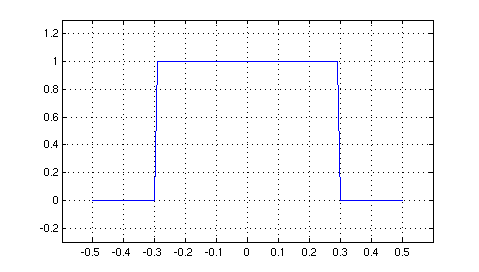
\includegraphics[height=3cm]{img/passabasso.png}
\caption{$\mid H(f) \mid$ di un filtro passabasso con $f_t=0.3$}
\end{figure}
\\
Esempio: passa alto ideale
$$ \mid H(f) \mid = 1-\mbox{rect}\Bigr(\frac{f}{2f_t}\Bigr) \quad \mbox{con } f_t<\frac12$$
Esempio: mediatore
$$ h[n]=\mbox{rect}_N\Bigr[n+\frac N2\Bigr] $$
supponendo N pari:
\begin{align*}
	H(f) &= \sum_{n=-\infty}^{\infty}h[n]\cdot \exp(-j2\pi fn)=\\
	&= \sum_{n=-\frac N2}^{\frac N2-1}\exp(-j2\pi fn)=\\
	&= \exp\Bigr(-j2\pi f\Bigr(-\frac N2\Bigr)\Bigr) + \exp\Bigr(-j2\pi f\Bigr(-\frac N2+1\Bigr)\Bigr)+
		\dots + \exp\Bigr(-j2\pi f\Bigr(\frac N2-1\Bigr)\Bigr)=\\
	&= \exp(j\pi fN)\Bigr[ 1+\exp(-j2\pi f)+\dots+\exp(-j2\pi f(N-1)) \Bigr]= \qquad \mbox{serie geometrica}\\
	&=\exp(j\pi fN)\cdot\frac{1-[\exp(-j2\pi f)]^{N-1+1}}{1-\exp(-j2\pi f)} =\\
	&= \frac{\exp(j\pi fN)-\exp(-j\pi fN)}{2j}\cdot\frac{2j}{\exp(j\pi f)-\exp(-j\pi f)}\cdot\frac{1}{\exp(-j\pi f)}=\\
	H(f)&=\frac{\sin(\pi fN)}{\sin(\pi f)}\cdot\exp(j\pi f)
\end{align*}
\\
$\mid H(f) \mid$ si annulla in ogni multiplo di $\frac1N$
\begin{figure}[htp]
\centering
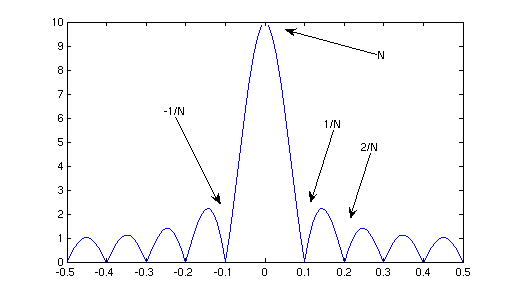
\includegraphics[height=4cm]{img/mod-mediatore.png}
\caption{$\mid H(f) \mid$ di un mediatore con $N=10$}
\end{figure}
\\
$\arg(H(f))=\pi f + \pi \cdot \mbox{sgn} \Bigr( \frac{\sin(\pi fN)}{\sin(\pi f)} \Bigr)$

\section{DTFT Discrete Time Fourier Transform}
$$ x[n] \longleftrightarrow X(f)=\sum_{n=-N}^{N}x[n]\cdot \exp(-j2\pi fn) $$
$X(f)$ \'e una funzione \emph{continua} $\in R$\\
\\
La convoluzione lineare nel dominio dei tempi diventa un prodotto nel dominio delle frequenze. Ad esempio,
nello studio di sistemi LTI:
\begin{align*}
	x[n] &\longrightarrow y[n]=x[n]*h[n]\\
	X(f) &\longrightarrow Y(f)=X(f)\cdot H(f)\\
	&\downarrow\\
	Y(f) &\longrightarrow \mid X(f) \mid \cdot \mid H(f) \mid \cdot \exp(\mbox{arg }X(f) + \mbox{arg }H(f))\\
	&\downarrow\\
	\mid Y(f) \mid &= \mid X(f) \mid \cdot \mid H(f) \mid &\mbox{risposta in ampiezza}\\
	&\downarrow\\
	\mbox{arg }(Y(f)) &= \mbox{arg }X(f)+\mbox{arg }H(f) &\mbox{risposta di fase}\\
\end{align*}

\subsection{Esistenza della DTFT
}
Condizione \emph{sufficiente} per l'esistenza \'e l'assoluta sommabilit\'a di $x[n]$
$$ \sum_{n=-\infty}^{\infty}\mid x[n]\mid < \infty $$
Poich\'e:
$$ \mid \sum_{n=-\infty}^{\infty} x[n]\exp(-j2\pi fn) \mid \leq 
	\sum_{n=-\infty}^{\infty}\mid x[n]\mid \cdot \mid \exp(-j2\pi fn)\mid \leq
	\sum_{n=-\infty}^{\infty}\mid x[n] \mid
$$
In tal caso $X(f)$ esiste al senso della funzione.\\
\\
Pu\'o anche succedere che $x[n]$ sia a energia finita ma non assolutamente sommabile.
$$ W_x = \sum_{n\in Z} \mid x[n] \mid^2 < \infty \quad \mbox{ma } \alpha\rightarrow\infty $$
Per esempio:
\begin{align*}
	x[n] &= A\cdot \mbox{sinc}(2f_tn)\\
	&\updownarrow\\
	X(f) &= \frac{A}{2f}\mbox{rect}\Bigr( \frac{f}{2f_T} \Bigr) & \mid f \mid<\frac{1}{2}, 0<f_T<\frac12
\end{align*}
Altro caso: $x[n]$ a potenza media finita non nulla (quindi energia infinita).
In tal caso $X(f)$ pu\'o esistere ma in generale solo al senso delle distribuzioni.\\
Per esempio:
\begin{align*} 
	x[n]&=\cos(2\pi f_0n)\\
	&\updownarrow\\
	X(f)&= \frac 12[\delta_1(f+f_0)+\delta_2(f-f_0)]
\end{align*}


\subsection{Convergenza della DTFT}
Se definisco una DTFT svolta solo su una parte del segnale nei tempi (2M+1 campioni):
\begin{align*} 
	X_M(f) &= \sum_{m=-M}^{M} x[m]\cdot\exp(-j2\pi fm)\\
	&= \DTFT(x[m]\cdot\mbox{rect}_{2M+1}[m+M])
\end{align*}
In tal caso la DTFT converge in generale (per $X(f)$ funzioni) solamente in \emph{media quadratica}.
$$ \lim_{M\to\infty} \int_{u}^{u+1} \mid X(f) - X_M(f)\mid^2\,df=0 $$
Di conseguenza si presentano i \emph{fenomeni di gibbs} quando si finestrano (con $M<\infty$) sequenze
che hanno discontinuit\'a di prima specie in $X(f)$.\\\\
Esempio:
\begin{align*}
	x[n] &= 2f_t\cdot\sinc(2f_tn)\\
	\\
	X_M(f) &= \DTFT(2f_t\cdot\sinc(2f_tn)\cdot\rect_{2M+1}[n+m])\\
	&= \DTFT(2f_t\cdot\sinc(2f_tn))\convcirc_1\DTFT(\rect_{2M+1}[n+m])\\
	&= \rect\Bigr( \frac{f}{2f_t} \Bigr) \convcirc_1 \frac{\sin(\pi f(2M+1))}{\sin(\pi f)}\\
	&= \int_{-f_t}^{f_t}\frac{\sin(\pi f(2M+1))}{\sin(\pi f)}\,df
\end{align*}
La convergenza non uniforme porta (nel caso di discontinuit\'a, come nel finestramento con un rect) a della
oscillazioni, per quanto grande sia M.


\subsection{Propriet\'a della DTFT}
\begin{enumerate}
	\item Periodica di periodo 1
	
	\item Linearit\'a\\
	$\forall x_1[n],x_2[n],\quad \alpha_1,\alpha_2 \in C$
	$$ \alpha_1\cdot x_1[n]+\alpha_2\cdot x_2[n] \longleftrightarrow \alpha_1\cdot X_1(f)+\alpha_2\cdot X_2(f) $$

	\item Hermitianit\'a
	$$ x^*[n] \longleftrightarrow X^*(f) $$
	Quindi un segnale reale nei tempi ha trasformata con parte reale pari e parte immaginaria dispari.

	\item Traslazione/modulazione
	$$ x[n] \longleftrightarrow X(f) $$
	\begin{align*}
		x[n-n_0]&\longleftrightarrow X(f)\cdot\exp(-j2\pi fn_0)&\mbox{Traslazione nei tempi}\\
		\\
		x[n]\cdot\exp(j2\pi f_0n)&\longleftrightarrow X(f-f_0)&\mbox{Modulazione nei tempi}		
	\end{align*}
	
	\item Moltiplicazione/convoluzione
	\begin{itemize}
		\item Moltiplicazione
		\begin{align*}
			x_1[n]\cdot x_2[n] \longleftrightarrow & X_1(f) \otimes_1 X_2(f) &\mbox{Moltiplicazione}\\
				& \int_{u}^{u+1}X_1(f')\cdot X_2(1-f')\,df'
		\end{align*}
		Dimostrazione:
		\begin{align*}
			x[n]&= \mbox{DTFT}^{-1}(X_1(f)\otimes_1 X_1(f))=\\
			&=\int_{u}^{u+1}\Bigr[\int_{v}^{v+1}X_1(f')\cdot X_2(f-f')\,df'\Bigr]\cdot \exp(j2\pi fn)\,df=\\
			&=\int_{f'=v}^{v+1}X_1(f')\cdot\Bigr[
				\underbrace{ \int_{f=u}^{u+1}X_2(f-f')\cdot\exp(j2\pi fn)\,df \Bigr]}_
					{x_2[n]\cdot\exp(-j2\pi f'n)}
			\,df'=\\	
			&=x_2[n]\cdot\int_{f'=v}^{v+1}X_1(f')\cdot\exp(-j2\pi f'n)\,df'\\
			&=x_1[n]\cdot x_2[n]
		\end{align*}
	
		\item Convoluzione lineare
		\begin{align*}
			x_1[n]*x_2[n] &\longleftrightarrow X_1(f)\cdot X_2(f) &\mbox{Convoluzione lineare}
		\end{align*}
		Dimostrazione:
			$$\sum_{n=-\infty}^{\infty}\Bigr( \Bigr( \sum_{m=-\infty}^{\infty} x_1[m]x_2[n-m] \Bigr)
				\cdot\exp(-j2\pi fn) \Bigr)=$$
			$$ \sum_m x_1[m] \Bigr(\underbrace{\sum_n x_2[n-m] \cdot \exp(-j2\pi fn)}_
				{X_2(f)\cdot \exp(-j2\pi fm)}			
			\Bigr)= $$
			$$ X_2(f) \cdot\underbrace{\sum_m x_1[m]\cdot\exp(-j2\pi fm)}_
				{X_1(f)}
			= $$
			$$X_2(f)\cdot X_1(f)$$
	\end{itemize}

	\item
		\begin{itemize}
			\item $x[n]$ \'e pari $\Rightarrow$ X(f) \'e pari \\\\
				$x[n]$ \'e reale pari $\Rightarrow$ X(f) \'e reale pari\\\\
				$x[n]$ \'e coniugato pari $\Rightarrow$ X(f) \'e coniugato pari\\\\
				$ x[n]=x^*[-n] $
			\item $x[n]$ \'e dispari $\Rightarrow$ X(f) \'e dispari \\\\
				$x[n]$ \'e reale dispari $\Rightarrow$ X(f) \'e puramente immaginaria e dispari\\\\
				$x[n]$ \'e coniugato dispari $\Rightarrow$ X(f) \'e coniugato dispari\\\\
				$ x[n] = -x^*[-n] $
		\end{itemize}
	
	\item Teorema di Parseval:
		$$ W_x = \sum_{m=-\infty}^{\infty}\mid x[m] \mid^2 \quad = \quad \int_{u}^{u+1}\mid X(f) \mid^2 \, df $$
		\begin{align*} 
			<x,y^*> \quad &=\quad \int_{u}^{u+1} X(f)\cdot Y^*(f)\, df \quad \\
			&\stackrel{\triangle}{=} \quad \sum_{m=-\infty}^{\infty}x[m]\cdot y^*[m]
		\end{align*}
		IMPORTANTE: $X(f)$ NON \'e a energia finita! Lo \'e solo su un periodo per sequenze a energia finita.

	\item Ribaltamento
		\begin{align*}
			x[n] &\leftrightarrow X(f)\\
			x[-n] &\leftrightarrow X(-f)
		\end{align*}

	\item 
		$$ n\cdot x[n] \quad \Longleftrightarrow \quad \frac{j}{2\pi}\cdot\frac{dX(f)}{df} $$
		Dimostrazione:
		\begin{align*}
			X(f) &= \sum_{n\in Z}x[n]\cdot \exp(-j2\pi fn)\\
			\frac{dX}{df} &= \sum_{n\in Z} x[n]\cdot [ -j2\pi n \cdot \exp(-j2\pi fn) ]\\
			&= \sum_{n\in Z} -j2\pi n\cdot x[n] \cdot \exp(-j2\pi fn)\\
			\\
			-j2\pi n\cdot x[n] \quad &\Longleftrightarrow \quad \frac{dX(f)}{df}\\
			\\
			n\cdot x[n] \quad &\Longleftrightarrow \quad \frac{1}{-j2\pi}\cdot\frac{dX(f)}{df} =
				\frac{j}{2\pi}\cdot \frac{dX(f)}{df}
		\end{align*}

\end{enumerate}

\subsection{Formula di inversione:}
\begin{align*}
	X(f)&= \sum_n x[n]\cdot\exp(-j2\pi fn)\\
	\updownarrow&\\
	x[n]&= \int_{u}^{u+1}X(f)\cdot\exp(j2\pi fn)\,df\qquad \forall u \in R
\end{align*}
La formula si dimostra a partire dalla Trasformata di Fourier di $X(f)$ (periodo 1)
$$ X(f) = \sum_{k=-\infty}^{\infty} x_k\cdot\exp\Bigr( j2\pi \frac k1f \Bigr) $$
$$ x_k = \frac11 \int_{u}^{u+1} X(f)\cdot\exp\Bigr( -j2\pi \frac K1 f \Bigr) $$

\subsection{DTFT della crosscorrelazione lineare di sequenze}
$$ \varphi_{xy}[n] \quad \stackrel{\triangle}{=} \quad\sum_{m\in Z} x^*[m]\cdot y[n-m] $$
$$ \varphi_{xy}[n]=x^*[-n]*y[n] \quad\Longleftrightarrow\quad X^*(f)\cdot Y(f) $$

\subsection{Coppie sequenze - DTFT}
\begin{align*}
	\delta[n] \quad &\longleftrightarrow \quad 1\\
	x[n]=1 \quad \forall n \quad &\longleftrightarrow \quad \delta_1(f)=\sum_{k\in Z}\delta(f-k)\\
	a^n\cdot\varepsilon[n] \quad &\longleftrightarrow \quad \frac{1}{1-a\cdot \exp(-j2\pi f)} \quad \mid a\mid < 1\\
	\varepsilon[n] \quad &\longleftrightarrow \quad \frac{1}{1-\cdot \exp(-j2\pi f)}+\frac 12 \delta_1(f)\\
	(n+1)a^n \cdot \varepsilon[n] \quad &\longleftrightarrow \quad \frac{1}{[1-a\cdot \exp(-j2\pi f)]^2}\\
	\mbox{rect}_N(n) \quad &\longleftrightarrow \quad \frac{\sin(\pi fn)}{\sin(\pi f)} &\mbox{N dispari}\\
		\quad &\longleftrightarrow \quad \frac{\sin(\pi fn)}{\sin(\pi f)}\cdot\exp(-j\pi f) &\mbox{N pari}\\
	2f_t\cdot \mbox{sinc}(f_t\cdot n) \quad 0<f_t<\frac 12\quad &\longleftrightarrow \quad \mbox{rect}\frac{f}{2f_t} 
		\quad \mbox{ripetizione periodo 1}\\
	\mbox{filtro passabasso ideale}
\end{align*}
Dimostrazione:
\begin{align*}
	S(f) &= \mbox{rect}\frac{f}{2f_t} \quad \mid f \mid < \frac 12\\
	s[n] &= \int_{-\frac 12}^{\frac 12} \mbox{rect}\frac{f}{2f_t}\cdot\exp(j2\pi fn)\, df\\
	&= \int_{-f_t}^{f_t}\exp(j2\pi fn)\, df \\
	&= \frac{1}{j2\pi fn}\cdot\exp(j2\pi fn)\mid_{-f_t}^{f_t}\\
	&= \frac 1{\pi n}\sin{2\pi f_tn} \quad = \quad 2\cdot f_t\cdot\mbox{sinc}(2f_t n)
\end{align*}

\section{Campionamento e ricostruzione}

\subsection{Campionamento ideale}
Si normalizza l'asse delle frequenze rendendo periodica di periodo 1 la trasformata.
\begin{center}
	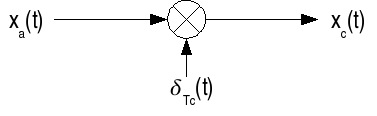
\includegraphics[height=2cm]{img/campionamento.jpg}\\
	$T_c$: periodo di campionamento
\end{center}
$$ x_c(t) = x_a(t)\cdot\delta_{T_c}(t)=x_a(t)\cdot\sum_{k\in Z}\delta(t-kT_c)=\sum_{k\in Z}x_a(kT_c)\cdot\delta(t-kT_c) $$
$$ \delta_{T_c}(t) \longleftrightarrow \frac{1}{T_c}\delta_{\frac{1}{T_c}}(f)$$
\begin{align*}
	F\{x_c(t)\}&=F\{ x_a(t)\cdot \delta_{T_c}(t) \}\\
	&= X_a(f)*\frac{1}{T_c}\delta_{\frac1{T_c}}(f)\\
	&= \frac1{T_c}\sum_{k\in Z} X_a\Bigr( f-\frac k{T_c} \Bigr)
\end{align*}
Campionamento nei tempi significa periodicizzazione dello spettro di frequenza.
\begin{center}
	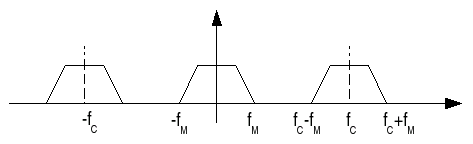
\includegraphics[height=2.5cm]{img/campionamento2.png}
\end{center}
Aliasing: sovrapposizione delle ripetizioni spettrali quando $f_c-f_M>f_c$, si elimina imponendo $f_c>2f_M$\\
\\
Dunque, sappiamo che:
$$ X_c(f)=\frac1{T_c}\cdot\sum_{n\in Z} X_a(f-nf_c) $$
sappiamo anche che:
\begin{align*} 
	x_c(t) &= \sum_{n\in Z}x_a(nT_c)\cdot\delta(t-nT_c)\\
	&\updownarrow\\
	X_c(f) &= \sum_{n\in Z} X_a(nT_c)\cdot\exp(-j2\pi f_nT_c)
\end{align*}
Supponendo $x[n]$ versione campionata di $x_a(t)$ con periodo $Tc$:
$$ x[n]=x_a(t) \mid_{t=nT_C} = x_a(nT_c) $$
Sapendo che:
$$ x[n] \leftrightarrow X(f)=\sum_{n\in Z} x[n]\cdot\exp(-j2\pi fn) $$
Scopriamo le due equazioni (equivalenti):
\begin{align*}
	X_c(f) &= X(f\cdot T_c)\\
	X(f) &= X_c(f\cdot f_c)
\end{align*}
Interpretazione: la DTFT \'e la versione riscalata della trasformata di Fourier del segnale campionato
di un fattore $f_c$.
$$ X(fT_c)=\frac1{T_c}\sum_{n\in Z} X_a\Bigr(f-\frac n{T_c}\Bigr) $$
$$ X(f) = \frac 1{T_c}\sum_{n\in Z} X_a \Bigr( \frac{f-n}{T_c} \Bigr) $$

\subsection{Ricostruzione del segnale}
Supponiamo assenza di aliasing. Un ricostruttore deve avere la seguente funzione di trasferimento:
\begin{align*}
	\mid G_r(f) \mid &= Tc &f\in[-f_M,f_M]\\
		&= 0 &kf_c-f_M<f<kf_c+f_M \quad k\in Z^*\\
		&= qualsiasi &altrove\\\\
	\mbox{arg}(G_r(f)) &\mbox{ nullo o a fase lineare }(-j2\pi ft_0) &\mbox{ (introduce al pi\'u un ritardo)}
\end{align*}
\begin{center}
	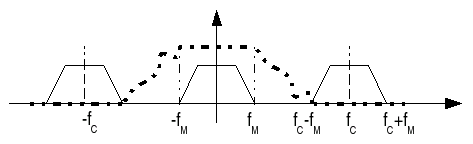
\includegraphics[height=2.5cm]{img/ricostruzione.png}
\end{center}
Caso particolare:
\begin{align*}
	\mid G_r(f) \mid &= T_c\cdot\rect\Bigr(\frac{f}{f_c}\Bigr)\\
	g_r(t) &= \sinc(f_c(t-t_0))&t_0=0\\
	x_a(t) &= g_r(t)*x_c(t) = \sum_{k}x_a(kT_C)\cdot\sinc(f_ct-k)
\end{align*}
\clearpage
Esempio: segnale audio $x_a(t)$ con $f_M=20KHz$ e $f_c=44.1KHz$.
\begin{figure}[h]
	\centering
	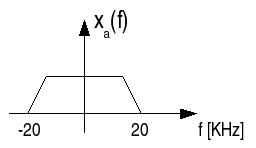
\includegraphics[height=2.5cm]{img/ricostruttoreaudio01.png}
	\caption{Spettro del segnale di partenza}
	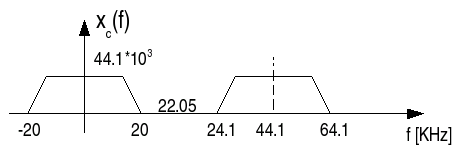
\includegraphics[height=2.5cm]{img/ricostruttoreaudio02.png}
	\caption{Spettro del segnale di partenza campionato}
	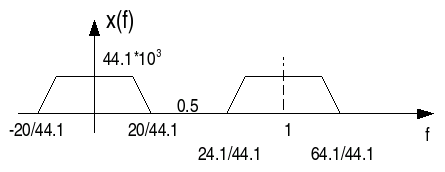
\includegraphics[height=2.5cm]{img/ricostruttoreaudio03.png}
	\caption{DTFT del segnale di partenza campionato}
	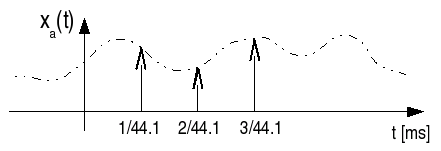
\includegraphics[height=2.5cm]{img/ricostruttoreaudio04.png}
	\caption{Segnale campionato}
\end{figure}

\noindent Rispettando le regole viste prima per avere un ricostruttore ideale, sono possibili infiniti algoritmi. Ad esempio:
\begin{align*}
	G_{r1} &= T_c\cdot\rect\Bigr(\frac{f}{f_c}\Bigr)\\
	g_{r1} &= \sinc(f_ct)\\
	\\
	G_{r2} &= T_c\cdot\rect\Bigr( \frac f{2f_M} \Bigr)\\
	g_{r2} &= \underbrace{2f_M T_c}_
		{0.9}
	\cdot \sinc(\underbrace{2f_M}_
		{40000}
	t)
\end{align*}

\noindent Entrambi questi ricostruttori sono in grado di ricostruire perfettamente il segnale di partenza.

\clearpage

\subsection{Campionamento reale}
\begin{figure}[h]
	\centering
	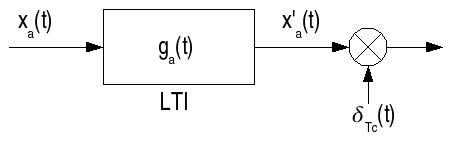
\includegraphics[height=2.5cm]{img/campionamentoreale.png}
\end{figure}
$g_a(t)$ \'e un filtro integratore (sample\&hold), serve  integrare il segnale analogico in un piccolo intorno dell'istante di campionamento. Tipicamente:
\begin{align*}
	g_a(t) &= \rect\Bigr( \frac t\Delta \Bigr)\\
	x'_a(t) &= x_a(t)*g_a(t) \\
	&= \frac 1\Delta \int_{\frac \Delta 2}^{-\frac \Delta 2} x_a(t) \,dt
\end{align*}
\begin{align*}
	x_{c_{reale}}(t) \longleftrightarrow X_{c_{reale}}(f)&=\frac1{T_c}\delta_{T_c}(f)*[X_a(f)\cdot G_a(f)]\\
	&= \frac1{T_c}\sum_{n \in Z}X_a\Bigr( f-\frac n{T_c} \Bigr) \cdot G_a\Bigr( f-\frac n{T_c} \Bigr)
\end{align*}

\noindent Esempio: $ G_a(f) = \sinc(\Delta f) $\\
$X'_a(f) = X_a(f)\cdot G_a(f)$ risulta leggermente deformato.
\begin{figure}[h]
	\centering
	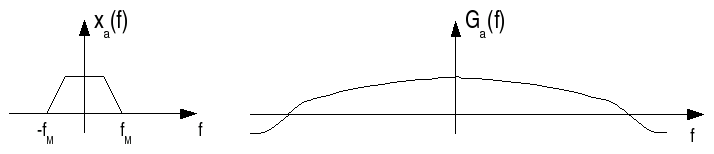
\includegraphics[height=2.5cm]{img/campionamentoreale2.png}
\end{figure}

$$ X_{c_{reale}}(f) = \frac1T_c \sum X_a\Bigr( f-\frac KT_c \Bigr)\cdot T_c\cdot \sinc(fT_c)\cdot\underbrace{\exp(-j2\pi fT/2)}_
	{\mbox{uscita ritardata di 1/2 campione}} $$

Non c'\'e alcun cambiamento per quanto riguarda l'aliasing ($f_c$ deve rimanere $>2f_M$), ma la
ricostruzione deve tenere conto della deformazione.

\begin{align*}
	\mid G_r(f) \mid &= \frac{T_c}{\mid G_a(f) \mid} &f\in[-f_M,f_M]\\
		&= 0 & kf_c-f_M < f < kf_c+f_M \quad k \in Z^*\\
		&= qualsiasi & altrove
\end{align*}


\subsection{Interpolatore lineare}
Equivale a due sample\&hold in cascata. L'uscita \'e dunque ritardata di 1 campione.
$$\huge{disegno}$$
$$ h(t)=\tri\Bigr( \frac{t-T}{T} \Bigr) $$
\begin{align*}
	x_c(t) &= x_a(t)\cdot\delta_T(t)*h(t)\\
	&\updownarrow\\
	X_c(f) &= \sum_k X_a\Bigr(f-\frac KT\Bigr)\cdot T\cdot \sinc^2(fT)\cdot\exp(-j2\pi fT)
\end{align*}
Lo spettro \'e molto simile, e il filtro ricostruttore \'e:
$$ H_r(f) = \frac 1{\sinc^2(fT)}\cdot\rect\frac ff_c $$




\clearpage

\section{Conversione digitale-digitale}
Si pu\'o vedere come un sistema lineare tempovariante.
\SISTEMA{$x[n]$}{$g_m[n]$}{$y[m]$}
Esempio: cambio del periodo di campionamento da $T_c$ a $T'_c$
$$ \frac{T'_c}{T_c}=\frac{M}{L} $$
$$ x_a(t)=\sum_n x[n]\cdot\sinc(f_ct-n) \quad \mbox{con filtro di ricostruzione ideale} $$
\begin{align*}
	y[m] &= x_a(t)\mid_{t=mT'_c}=\\
	&= \sum_n x[n]\cdot\sinc\Bigr( m\frac{T'_c}{T_c}-n \Bigr)=\\
	&= \sum_n x[n]\cdot\sinc\Bigr( m\frac ML -n \Bigr)&\mbox{operazione puramente numerica}
\end{align*}

\begin{figure}[h]
	\centering
	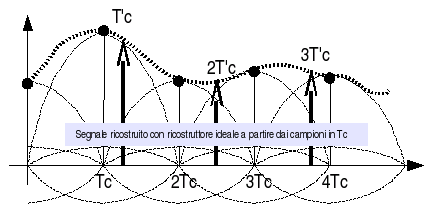
\includegraphics[height=5cm]{img/convdd.png}\\
\end{figure}

Con un generico filtro di ricostruzione con risposta all'impulso $\tilde g(t)$:
\begin{align*}
	\tilde x_a(t)&=\sum_n x[n]\cdot\tilde g(t-n)\\
	\tilde y[m]&=\sum_n x[n]\cdot\tilde g(mT'_c-n)&\mbox{una specie di convoluzione}
\end{align*}

Lo stesso procedimento pu\'o essere svolto interpolando e poi decimando il segnale di partenza:
\begin{figure}[h]
	\centering
	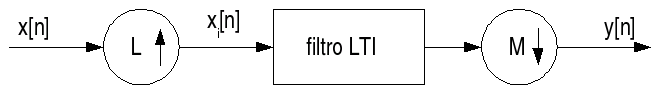
\includegraphics[height=1cm]{img/convdd2.png}\\
\end{figure}

\clearpage

\subsection{Decimazione numerica di fattore H}
$$ x_d[n]=x[n\cdot H] $$
$$ x[n] \stackrel{DTFT}{\longleftrightarrow} X(f) = \frac1{T_c}\sum_n x_a\Bigr( \frac{f-n}{T_c} \Bigr) $$
$$\downarrow$$
$$ x_d[n] \stackrel{DTFT}{\longleftrightarrow} X_d(f) = \frac1{H\cdot T_c}\sum_n x_a\Bigr( \frac{f-n}{H\cdot T_c} \Bigr) $$
(ripetizione di $X_a(f)$ ogni $f_c$ + cambio scala di un fattore $f_c$).\\
Svolgendo un paio di passaggi matematici si ha che:
\begin{align*}
	n &= i+kM\\
	X_d(f)&= \frac1{HT_c}\sum_k \sum_{i=0}^{M-1}x_a\cdot\Bigr( \frac{f-(1+kM)}{HT_c} \Bigr)=\\
	&= \frac1H \sum_{i=0}^{M-1}\underbrace{\Bigr( \frac1{T_c} \sum_k x_a\Bigr( \frac{\frac{f-i}{M}-k}{T_c} \Bigr) \Bigr)}_
		{X\Bigr( \frac{f-i}{M} \Bigr)}
		=\\
	&= \frac1M \sum_{i=0}^{M-1}X\Bigr( \frac{f-i}M \Bigr)
\end{align*}
(allargamento di $X(f)$ attorno a ciascuna posizione intera $\Rightarrow$ possibile aliasing)

\begin{figure}[h]
	\centering
	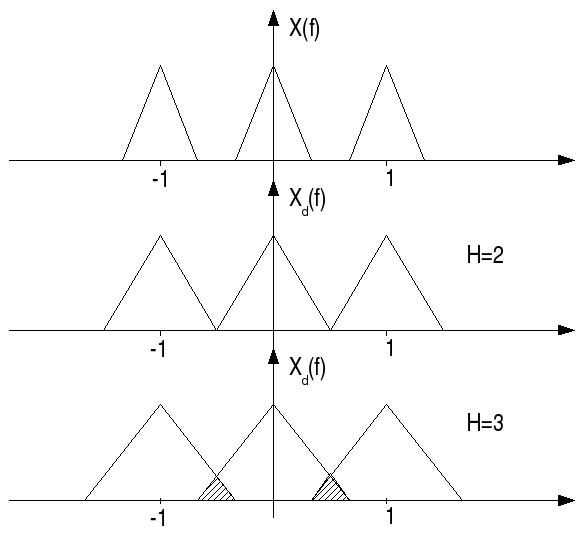
\includegraphics[height=8cm]{img/decimazionedigitale.png}\\
\end{figure}

(l'aliasing pu\'o essere evitato prefiltrando il segnale da decimare con un filtro con larghezza di banda $\frac1{2M}$)

\begin{figure}[h]
	\centering
	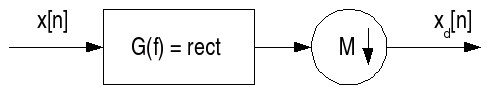
\includegraphics[height=1cm]{img/decimazionedigitale2.png}\\
\end{figure}

\clearpage

\subsection{Interpolazione numerica di fattore L}
\begin{align*}
	x_i[n]&=x[M/L]\qquad n=kL\quad k\in Z\\
	&=0 \qquad altrove
\end{align*}
\begin{align*}
	X_i(f) &= \sum_n x_i[n]\cdot\exp(-j2\pi fn)\\
	&= \sum_{n=kL} x[n/L]\cdot\exp(-j2\pi fn)\\
	&= \sum_k x[k]\cdot\exp(-j2\pi fkL)\\
	&=X(fL)
\end{align*}
Si verifica una compressione dell'asse delle frequenze di un fattore L (attorno a 0).\\

\begin{figure}[h]
	\centering
	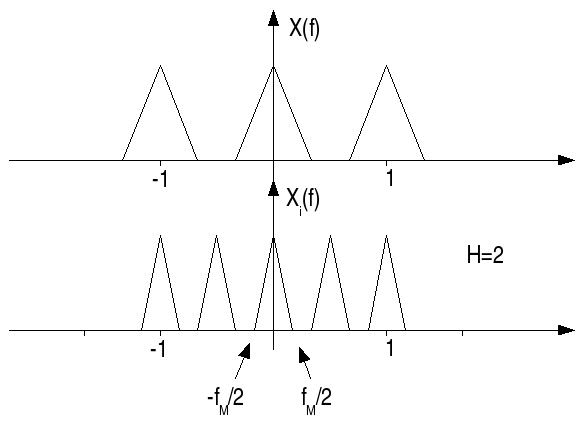
\includegraphics[height=6cm]{img/interpolazionedigitale.png}\\
\end{figure}

Si creano delle repliche di $X_a(f)$ ogni $1/L$. Queste repliche costituiscono un disturbo e devono essere 
eliminate, ad esempio con un filtro passabasso con frequenza di taglio $1/2L$.\\

\begin{figure}[h]
	\centering
	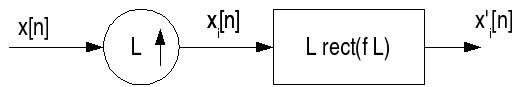
\includegraphics[height=1cm]{img/interpolazionedigitale2.png}\\
\end{figure}

Il guadagno L serve a correggere la perdita di energia dovuta alla compressione dell'asse delle frequenza.

\clearpage

\subsection{Interpolazione - decimazione in cascata}
\begin{figure}[h]
	\centering
	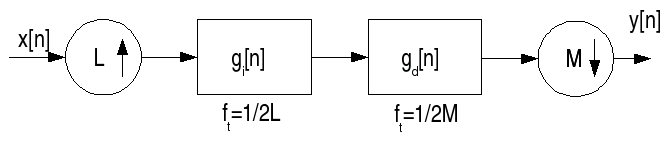
\includegraphics[height=1.5cm]{img/intdec1.png}\\
\end{figure}

Che \'e equivalente a dire\\:
\begin{figure}[h]
	\centering
	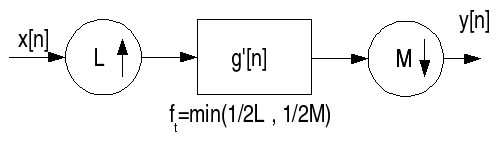
\includegraphics[height=1.5cm]{img/intdec2.png}\\
\end{figure}

Esempio: zoom di una immagine digitale di un fattore $2/3$ in altezza:\\
\begin{figure}[h]
	\centering
	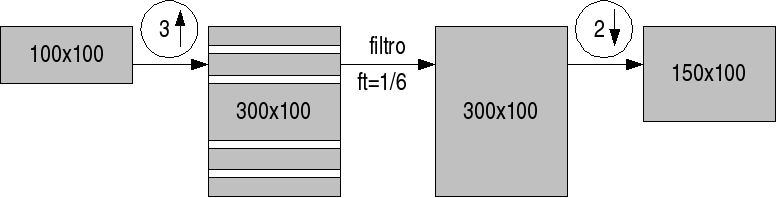
\includegraphics[height=2cm]{img/intdec3.png}\\
\end{figure}

\clearpage

\section{Trasformata Z}
La trasformata Z serve a gestire la convergenza della DTFT e a rappresentare i sistemi LTI descritti da
equazioni alle differenze.\\
\\
\emph{Definizione}: trasformata Z bilatera a variabile complessa $z$.
\begin{align*}
	X(z) &= \sum_{n=-\infty}^{\infty} x[n]\cdot z^{-n} \quad z\in C \\
	\downarrow &z = r\cdot \exp(j2\pi f)\\
	X(z) &= \sum_n (x[n]\cdot r^{-n})\cdot\exp(-j2\pi fn)
\end{align*}
La trasformata Z \'e periodica in f di periodo 1.\\
Inoltre da sopra si nota che quando $|r|=1$ la trasformata Z corrisponde alla DTFT.
\begin{figure}[h]
	\centering
	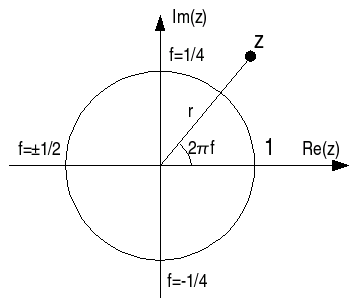
\includegraphics[height=4cm]{img/zeta01.png}
\end{figure}

\subsection{Condizioni di esistenza}
La trasformata Z converge in insiemi denominati ROC (region of convergence), ovvero l'insieme degli $z\in C$
tale che $\mid X(z) \mid$ converge.
$$ \mid X(z) \mid\quad \leq\quad \sum_{n=-\infty}^{\infty} \mid x[n] \mid\cdot z^{-n} \leq \quad\infty $$
Le ROC vengono determinate mediante il Criterio di Cauchy.
\subsubsection{Criterio di Cauchy}
$$ \sum_{n=0}^{\infty} u_n<\infty \quad \mbox{se}\quad \lim_{n\to\infty}\mid u_n\mid^{\frac 1n}<1 $$
La ROC assumer\'a forma:
$$ ROC:\{ z\in C \quad:\quad 0\leq R_{X_-} < r < R_{X_+} \leq \infty \} $$
Infatti, 
$$ \sum_{n=-\infty}^{\infty}\mid x[n]\cdot z^{-n} \mid\quad=
	\quad\sum_{n=0}^{\infty}\mid x[n]\cdot z^{-n} \mid\quad +
	\quad \sum_{n=0}^{\infty} \mid x[-n]\cdot z^{n} \mid $$
E quindi, studiando la convergenza secondo Cauchy:
$$ ROC:\{ z\in C \quad:\quad 0\quad \leq \quad \lim_{n\to\infty}\mid x[n] \mid^{\frac 1n} \quad <\quad \mid z\mid 
	\quad < \quad \frac 1{\lim_{n\to\infty}\mid x[n]\mid^{\frac 1n}}\quad \leq\quad\infty    \} $$
All'interno della ROC $X(z)$ \'e una funzione analitica derivabile infinite volte e la derivata \'e continua.\\
NB: la DTFT esister\'a se il cerchio unitario ($\mid z \mid = 1$) \'e compreso nella ROC e tutte le sue derivate
sono continue. Nota bene:
$$ x[n]=\exp(j2\pi f_0n) \stackrel{DTFT}{\longleftrightarrow} \delta_1(f-f_0) $$
$\mid z \mid = 1$ \emph{non} \'e nella ROC, tuttavia la DTFT esiste al senso delle distribuzioni.\\
In questi casi arriva a toccare la circonferenza di raggio unitario al limite.\\
\\
\emph{Caso particolare}: quoziente di polinomi
$$X(z)=\frac{P(z)}{Q(z)} \qquad \mbox{polinomi in z e C}$$
soluzioni $P(z) = 0$ sono dette \emph{zeri} $z_i$\\
soluzioni $Q(z) = 0$ sono dette \emph{poli} $p_i$
\\
\begin{itemize}
	\item La ROC non contiene mai poli.
	\item Se $h[n]$ \'e a durata finita (sistemi FIR) la ROC \'e tutto il piano tranne al pi\'u 0 e $\infty$
	\item Se $h[n]$ \'e right-sided (illimitata) allora
		$$ ROC=\{ z\in C \quad:\quad \max_i\mid p_i\mid\quad<\quad\mid z\mid\quad 
			\stackrel{<}{\leq} \quad\infty \} $$
		\begin{itemize}
			\item $\leq$ : causale
			\item $<$ : non causale
		\end{itemize}
	\item Se $h[n]$ \'e right-sided allora
		$$ ROC=\{ z\in C \quad:\quad 0 \quad \stackrel{<}{\leq}\quad\mid z\mid
			\quad<\quad \min_i \mid p_i \mid\quad \} $$
	\item Se $h[n]$ \'e illimitata la ROC \'e l'intersezione:
		$$ ROC=\{ z\in C \quad : \quad \mid p_i \mid \quad < \quad \mid z \mid 
			\quad < \quad \mid p_{i+1} \mid \} $$
		dove $\mid p_i+1\mid > \mid p_i \mid$\\\\
\end{itemize}

Con $N$ poli si avranno $N+1$ ROC possibili.
\begin{figure}[h]
	\centering
	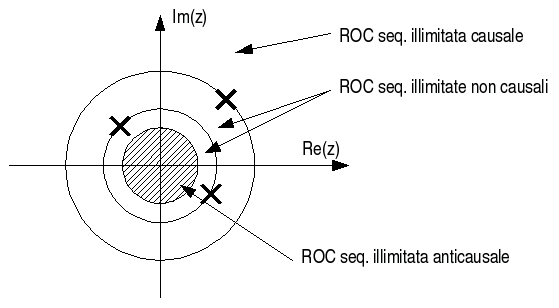
\includegraphics[height=4cm]{img/zeta02.png}\\
\end{figure}

\subsection{Trasformata inversa della Z}
\begin{enumerate} %inizio elenco numerato

	\item Integrale di Cauchy
		\begin{align*}
			\frac 1{2\pi j}\oint_{\Gamma}z^{l-1}\,dz \quad &= \quad 1 \quad \mbox{se } l=0 \quad l\in Z\\
			&= \quad 0 \quad \mbox{altrimenti}
		\end{align*}
		$\Gamma$: contorno chiuso che racchiude $z=0$.\\
		Si desidera calcolare lungo un contorno $\Gamma \in ROC$ che racchiude $z=0$ l'integrale:
		\begin{align*}
			I &= \frac 1{2\pi j}\oint_\Gamma X(z)\cdot z^{l-1}\,dz=\\
			&= \frac 1{2\pi j}\oint_\Gamma\Bigr( \sum_n x[n]\cdot z^{-n} \Bigr)\cdot z^{l-1}\,dz=\\
			&= \sum_n x[n]\cdot\frac 1{2\pi j} \oint_\Gamma z^{-n+l-1}\,dz=\\
			&= \sum_n x[n]\cdot [0 \mbox{ se } n\not= l,1 \mbox{ se } n=l]=\\
			&= x[l]\\
			&\downarrow\\
			x[n] &= \frac 1{2\pi j}\oint_\Gamma X(z)\cdot z^{n-1}\,dz\\
			&= \sum \mbox{residui}(X(z)\cdot z^{n-1}) \quad \mbox{in }\Gamma			
		\end{align*}
		\begin{itemize}
			\item residuo di un polo di ordine 1 in $z=a$ di $x(a)\cdot z^{n-1}$
				$$ \mbox{Res}^1_a=\lim_{z\to a} (z-a)\cdot X(z)\cdot z^{n-1} $$
			\item residuo di un polo di ordine $q$ in $z=a$ di $x(a)\cdot z^{n-1}$
				$$ \mbox{Res}^q_a = \lim_{z\to a} \frac1{(q-1)!} \cdot 
				\frac{d^{q-1}}{dz^{q-1}} \Bigr( x(a)\cdot z^{n-1}\cdot (z-a)^q \Bigr)$$
		\end{itemize}
		Esempio:
			$$ X(z)=\frac1{1-z^{-1}}\quad |z|>1 $$
			$$ X(z)\cdot z^{n-1}=\frac{z^n}{z-1} $$
			\begin{itemize}
				\item $n\geq 0$ : polo in $z=1$
				\item $n<0$ : polo in $z=1$ + polo di ordine $|n|$ in $z=0$
			\end{itemize}
			$$ \mbox{Res}_1^1=\lim_{z\to1} \frac{z^n}{z-1}(z-1)=1 $$
			$$ \mbox{Res}_0^1=\lim{z\to0} z\cdot\frac{z^{-1}}{z-1}=-1 $$
			$$ \mbox{Res}_0^{|n|}=\lim_{z\to0}\frac1{(|n|-1)!}\cdot\frac{d^{|n|-1}}{dz^{|n|-1}}
				\Bigr[ \frac{z^{-n}z^n}{z-1} \Bigr]= \lim_{z\to0}\frac1{(|n|-1)!}(-1)^{|n|-1}
				\cdot \frac{(|n|-1)!}{(z-1)^{|n|}}=-1$$
			\begin{align*}
				x[n] &= \sum \mbox{residui(polo z=1)}=1 &n\geq 0\\
				x[n] &= \sum \mbox{residui(poli z=1, |n|)}=1-1=0 &n<0
			\end{align*}
	
	\item Metodo per ispezione
		$$ X(z)=\frac 1{1-a^{-1}z} \quad\longleftrightarrow\quad x[n]=a^n\cdot\varepsilon[n] \qquad 
			\mid z\mid>\mid a\mid$$
		\begin{align*}
			X(z)=\sum_i X_i(z)&\\
			&X_i(z) \longrightarrow x_i[n]\\
			x[n]=\sum_i x_i[n]&
		\end{align*}

	\item Sviluppo in serie di frazioni parziali
		\begin{align*}
			X(z) &= \frac{P(z)}{Q(z)} = \frac{c\cdot\prod_{i=1}^{M}(z-z_i)}{\prod_{i=1}^{N}(z-p_i)}=\\
			&= c\cdot z^{M-N}\cdot\frac{\prod_{i=1}^{M}(1-z_i\cdot z^{-1})}{\prod_{i=1}^{N}(1-p_i\cdot z^{-i})}
		\end{align*}
		\begin{itemize}
			\item se $N>M$ e i poli hanno molteplicit\'a singolare:
				$$ X(z)=\sum_{i=1}^{N}\frac{A_i}{1-p_i\cdot z^{-i}} $$
				$$ A_i=(1-p_i\cdot z^{-1})\cdot X(z)|_{z=p_i} $$
			\item se $M>N$ e i poli hanno molteplicit\'a singolare:
				$$ X(z)=\sum_{i=1}^{M-N}B_i\cdot z^{-i}+\sum_{i=1}^{N}\frac{A_i}{1-p_i\cdot z^{-i}} $$
				Ove $B_i$ \'e la divisione polinomiale tra $P(z)$ e $Q(z)$ arrestata con grado
				resto $<N$.
			\item un polo $p_0$ con molteplicit\'a 2, $M \geq N$
				$$ X(z)=\sum_{i=1}^{M-N}B_i\cdot z^{-1}+\sum_{i=1}^{N-q}
					\frac{A_i}{a-p_i\cdot z^{-1}} + \sum_{i=1}^{q} \frac{C_i}
					{1-p_0\cdot z^{-i}}$$
				$$ C_i = \frac 1{(q-1)!\cdot(-p_0)^{q-1}}\cdot\Bigr( \frac{dq^{-i}}{d\omega^{q-1}}
					\cdot \Bigr( (1-p_0\omega)^q \cdot X(\omega^{-1}) \Bigr)\Bigr) \quad
					\omega = p_0^{-1}$$
		\end{itemize}

	\item Espressione in serie di potenze
		\begin{align*}
			X(z) &= z^2-\frac12z+-1+\frac12z^{-i}\\
			&\downarrow\\
			x[n] &= \delta[n+2]-\frac12 \delta[n+1]+\dots
		\end{align*}

	\item Divisione polinomiale
		$$ X(z)=\frac1{1-a\cdot z^{-1}} \qquad |z|>|a|$$
		(conosco $x[n]=a^n\cdot\varepsilon[n]$)
		\begin{itemize}
			\item soluzione causale:\\
				ordino in serie \emph{crescente} gli $z^{-1}$\\
				si effettua la divisione tra polinomi e si ottiene
				\begin{align*}
					&\sum_{0}^{\infty}1\cdot a^n\cdot z^{-n}\\
					&\updownarrow\\
					&x[n] = a^n\varepsilon[n]
				\end{align*}
			\item soluzione anticausale:\\
				ordino in serie \emph{crescente} gli $z$
				$$ X(z)=\frac z{z-a} $$
		\end{itemize}

\end{enumerate} %fine elenco numerato


\subsection{Propriet\'a della trasformata Z}

\subsubsection{Linearit\'a}
$\forall x_1[n],x_2[n], \alpha_1,\alpha_2\in C$
$$ x_1[n] \trasfz X_1(z)\quad ROC_1 $$
$$ x_2[n] \trasfz X_2(z)\quad ROC_2 $$
se $ROC_1 \cap ROC_2 \not= \emptyset$
$$ \alpha_1x_1[n]+\alpha_2x_2[n] \trasfz \alpha_1X_1(z)+\alpha_2X_2(z) $$
$$ ROC_1 \cap ROC_2 \subset ROC $$

\subsubsection{Traslazione}
$$ x[n]\trasfz X(z) $$
$$ x[n-n_0] \trasfz X(z)\cdot z^{-n_0} $$
Dimostrazione:
$$ \sum_n x[\underbrace{n-n_0}_{=m}]\cdot z^{-n} = \sum_m x[m]\cdot 
	\underbrace{z^{-(m+n_0)}}_{z^{-m}\cdot z^{-n_0}} = z^{-n_0}\cdot\sum_mx[n]\cdot z^{-m}=X(z)\cdot z^{-n_0} $$

\subsubsection{Cambio scala in Z}
$$ x[n]\trasfz X(z) $$
$$ ROC=\{ z\in C : R_{x^-}<|z|<R_{x^+} \} $$
\\
$$ a^n\cdot x[n]\trasfz X\Bigr( \frac wa \Bigr)\quad \mbox{con }w=az $$
$$ ROC=\{ w\in C : R_{x^-}-|a|<|z|<R_{x^+}+|a| \} $$
\begin{itemize}
	\item $0<|a|<1$ : avvicinamento di poli e zeri a $z=0$
	\item $|a|>1$ : allontanamento di poli e zeri da $z=0$
	\item $|a|=1$ : rotazione di $arg(a)$ di poli e zeri
\end{itemize}

\subsubsection{Derivazione in Z}
$$ n\cdot x[n]\trasfz -z\cdot\frac{dX}{dz} $$
La ROC rimane invariata a meno forse di $z=0$ e $z=\infty$.\\
Dimostrazione:
\begin{align*}
	\frac d{dz}X(z) &= \frac d{dz} \sum_n x[n]\cdot z^{-n}\\
	&= \sum_n x[n]\cdot\frac d{dz}(z^{-n})\\
	&= \sum_n x[n]\cdot(-n\cdot z^{-n+1})\\
	-\frac d{dz}X(z) &= \sum_n n\cdot x[n]\cdot z^{-1}\cdot z^{-n}
\end{align*}
Esempio:
$$ X(z) = \ln(1+az^{-1}) \qquad |z|>|a|$$
$$ \frac{dX}{dz}=\frac{-az^{-2}}{1+az^{-1}} $$
$$ -z\cdot\frac{dX}{dz}=\frac{az^{-1}}{1+az^{-1}}\trasfz \underbrace{a(-a)^{n+1}\cdot\varepsilon[n-1]}_
	{=nx[n]} $$
$$ Z^{-1}\{X(z)\}=\frac{a(-a)^{n-1}\cdot\varepsilon[n-1]}n=(-1)^{n-1}\cdot\frac{a^n}n \cdot\varepsilon[n-1] $$

\subsubsection{Coniugazione}
$$ x^*[n]\trasfz X^*(Z^*) $$

\subsubsection{Ribaltamento (sequenza)}
$$ x[n]\trasfz X(z)\qquad ROC=\{ z\in C : R_{x^-}<|z|<R_{x^+} \} $$
$$ x[-n]\trasfz X(z^{-1}) \qquad ROC=\{ z\in C : R_{x^+}<|z|<R_{x^-} \} $$
Dimostrazione:
$$ \sum_n x[-n]\cdot z^{-n} \quad m=-n \quad \sum_m x[m](z^{-1})^{-m}=X(z^{-1}) $$

\subsubsection{Convoluzione lineare di sequenze}
$$ x_1[n]\trasfz X_1(z)\quad ROC_1 $$
$$ x_2[n]\trasfz X_2(z)\quad ROC_2 $$
se $ROC_1 \cap ROC_2 \not= \emptyset$ allora:
$$ x_1[n]*x_2[n]\trasfz X_1(z)\cdot X_2(z) $$
$$ ROC_1 \cap ROC_2 \subset ROC $$
Dimostrazione:
\begin{align*}
	x_1[n]*x_2[n] &= \sum_n (x_1[n]*x_2[n])\cdot z^{-n} \\
	&= \sum_n \Bigr( \sum_m x_1[m]x_2[n-m] \Bigr) \cdot z^{-n}\\
	&= \sum_m x_1[m]\cdot \underbrace{\sum_n x_2[n-m]\cdot z^{-n}}_
		{X_2(z)\cdot z^{-m}}\\
	&= X_2(z)\cdot \underbrace{\sum_m x_1[m]\cdot z^{-m}}_
		{X_1(z)}
\end{align*}

\subsubsection{Moltiplicazione di sequenze}
\begin{align*}
	x_1[n]\cdot x_2[n] \trasfz& \frac1{2\pi j}\oint_{\Gamma_1}X_1(w)
		\cdot X_2\Bigr( \frac zw \Bigr)\cdot w^{-1}\,dw\\
	=&\frac1{2\pi j} \oint_{\Gamma_2}X_1\Bigr( \frac zw \Bigr)\cdot X_2(w)\cdot w^{-1}\,dw
\end{align*}
$\Gamma_1$: curva che racchiude $w=0$ e $\in \{ ROC_1\{w\}\cap ROC_2{z/w} \}$\\
$\Gamma_2$: curva che racchiude $w=0$ e $\in \{ ROC_1\{z/w\}\cap ROC_2{w} \}$

\subsection{Filtri FIR}
\begin{align*}
	h[n] &= 0 \quad n \not\in \{ n_0,n_0+1,\dots,N \}\quad N<\infty\\
	H[z] &= h[n_0]\cdot z^{-n_0}+h[n_0+1]\cdot z^{-n_0-1}+\dots &\mbox{Polinomio in z}
\end{align*}
Sistemi FIR: poli solo nell'origine (multipli), $N-1$ zeri.
\begin{itemize}
	\item Se $h[n]\in R$, numeratore della $H[z]$ \'e un polinomio a coefficienti reali.
	\item Cio\'e gli zeri di $H[z]$ sono necessariamente reali o complessi coniugati.
	\item Un polinomio di grado dispari ha sempre almeno uno zero reale.
\end{itemize}
$ ROC=C/ \{0\} $ solo se $h[n]$ \'e causale. Se $h[n]$ \'e anticausale $ROC=C/ \{\infty\}$.\\
\\
Un sistema LTI \'e stabile se e solo se $\sum_n |h[n]|<\infty$, e tutti i filtri FIR soddisfano
questa condizione.

\subsection{Filtri IIR}
$$ y[n]=\sum_{m\in Z}x[m]\cdot y[n-m] $$
\begin{itemize}
	\item Sistemi ARMA: rappresentabili con equazioni alle differenze.
	\item Sistemi non ARMA: non rappresentabili. Es: filtro passabasso ideale.
\end{itemize}
Nel caso di sistemi ARMA:
$$ \sum_{k=0}^{N}a_k\cdot y[n-k]=\sum_{l=0}^{M}b_l\cdot x[n-l] $$
Se $h[n]$ \'e causale:
$$ y[n]=-\sum_{k=1}^{N}\frac{a_k}{a_0}\cdot y[n-k]+\sum_{l=0}^{M}\frac{b_l}{a_0}\cdot x[n-l] $$
Calcolando la trasformata dei due membri:
$$ \sum_{k=0}^N a_k\cdot Y[z]\cdot z^{-k}=\sum_{l=0}^M b_l \cdot X[z]\cdot z^{-l} $$
$$ H[z]=\frac{Y[z]}{X[z]}=\frac{\sum_{l=0}^N b_l \cdot z^{-l}}{\sum_{k=0}^M a_k \cdot z^{-k}} $$
Di conseguenza un sistema ARMA pu\'o essere scritto cos\'i:
$$ H[z]=U[z]\cdot V[z]=\sum_{l=0}^N b_l\cdot z^{-l}\cdot \frac 1{\sum_{k=0}^M a_k\cdot z^{-k}} $$
\begin{itemize}
	\item $U[z]$: caratteristico di un sistema FIR (MA: moving average) (\emph{zeri})
	\item $V[z]$: parte auto regressiva AR (\emph{poli})
\end{itemize}
\SISTEMASERIE{$x[n]$}{$U[z]$ zeri}{$y_i[n]$}{$V[z]$ poli}{$y[n]$}
La parte AR non converge in prossimit\'a dei poli. \\
\\
Ci sono N poli complessi (reali o complessi coniugati).\\
\\
$N'$ poli con modulo diverso implica $N'+1$ regioni ROC. Ci sono $N'+1$ $h_s[n]$ diverse con la stessa
$H[z]$, tra le quali:
\begin{itemize}
	\item 1 causale (esterna) $|z|>\mod(p_i)$
	\item 1 anticausale (centro) $|z|<\mod(p_i)$
	\item tutte le altre non causali.
\end{itemize}
Stabilit\'a garantita se $H(z)$ converge in $z=\exp(j2\pi fz)$, nessun polo in $|z|=1$.	\\
\\
Nel caso ARMA:
$$ H(f)=H(z)\quad z=\exp(j2\pi f) $$
\begin{align*}
	|H(f)|&=|H_0\cdot \frac{\prod_{k=1}^M (1-c_k\cdot z^{-1})}{\prod_{k=1}^N (1-d_k\cdot z^{-1})} |\\
	&= |H_0|\cdot \frac{\prod_{k=1}^M |1-c_k\cdot z^{-1}|}{\prod_{k=1}^N |1-d_k\cdot z^{-1}|}\\
	\\
	\arg(H(f))&=\arg(I)|_{z=\exp(j2\pi f)}\\
	&= \arg(H_0)+\sum_{k=1}^M \arg(1-c_k\cdot z^{-1})-\sum_{k=1}^N\arg(1-d_k\cdot z^{-1})
\end{align*}


\subsection{Caratterizzazione di sistemi LTI}
\SISTEMA{$x[n]$}{$h[n]$ LTI}{$y[n]=x[n]*h[n]$}
$$Y(z)=X(z)\cdot H(z)$$
$$ H(f) = H(z)|_{z=\exp(j2\pi f)} \quad \mbox{se il sistema \'e stabile}$$
$$ |H(f)| =\frac{\prod || \mbox{vettori corrispondenti agli zeri} ||}{\prod || \mbox{vettori corrispondenti ai poli} || } \cdot |H_0|$$
$\arg H(f)=$ differenza tra la somma degli angoli formati dai vettori degli zeri, e la somma degli angoli dei vettori dei poli

\begin{figure}[h]
	\centering
	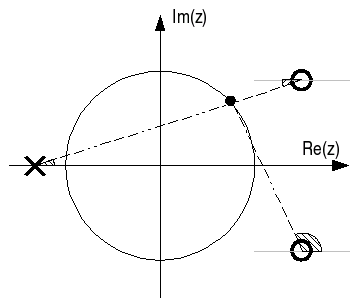
\includegraphics[height=4cm]{img/zeta03.png}\\
\end{figure}

\noindent Note:
\begin{itemize}
	\item uno zero su $\Gamma_1$ (cerchio unitario) $\Rightarrow$ $H(f)=0$ per f 
		corrispondente alla posizione dello zero.
	\item uno zero molto vicino a $\Gamma_1$ (rispetto agli altri poli e zeri) implica attenuazione massima
		di $|H(f)|$ per f tale che il punto sul cerchio sia a distanza minima dallo zero.
	\item un polo molto vicino a $\Gamma_1$ (rispetto agli altri poli e zeri) implica amplificazione massima
		di $|H(f)|$ per f tale che il punto sul cerchio sia a distanza minima dal polo.
\end{itemize}

\noindent Risposta all'impulso nota $H(z)$:
\begin{itemize}
	\item deve essere nota o desumibile la $ROC_H$
	\item invertire $H(z)$ con quella $ROC_H$
\end{itemize}
Risposta al gradino unitario nota $H(z)$:
\begin{itemize}
	\item deve essere nota o desumibile la $ROC_H$
	\item calcolare $H(z)\cdot\frac z{z-1}$ e invertire il tutto sulla $ROC_Y$
\end{itemize}

\subsection{Filtri passa tutto}

\subsubsection{Relazione tra modulo e fase}
\begin{align*}
	|G(f)|^2 = &G(f)\cdot G^*(f)\\
		&\updownarrow DTFT\\
		&g[n]*g^*[n]\\
		&\updownarrow Z\\
		&G(z)\cdot G\Bigr( \Bigr( \frac 1z \Bigr)^* \Bigr)\\\\
	|G(f)|^2 = &G(z)\cdot G^*({z^{-1}}^*)|_{z=\exp(j2\pi f)}
\end{align*}
Quindi, sistemi che ammettono la stessa $C(z)=G(z)\cdot G^*({z^{-1}}^*)$ ammettono la stessa risposta in ampiezza.\\
Nel caso ARMA:
$$ G(z)=G_0\cdot\frac{\prod_{k=1}^{M}(1-c_kz^{-1}) }{\prod_{k=1}^{N} (1-d_kz^{-1}) } $$
\begin{align*}
	&\downarrow\quad (a+b)^*=a^*+b^*\\
	&\downarrow\quad (ab)^*=a^*b^*
\end{align*}
$$ C(z)=|G_0|^*\cdot \frac{\prod_{k=1}^{M}(1-c_kz^{-1})(a-c_k^*z) }{\prod_{k=1}^{N}(1-d_kz^{-1})(a-d_k^*z) } $$
$C(z)$ ammette coppie coniugate e reciproche dei poli/zeri rispetto ai poli/zeri di $G(z)$.\\
\\
Esempio:
\begin{figure}[h]
	\centering
	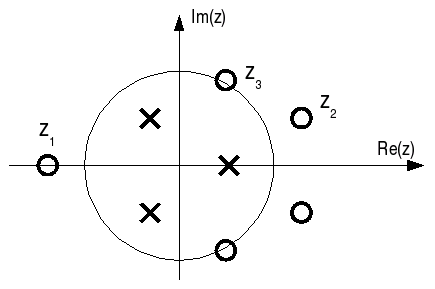
\includegraphics[height=4cm]{img/zeta04.png}\\
\end{figure}
Per sistemi causali e stabili, i poli di $C(z)$ interni al cerchio unitario sono anche poli di $G(z)$.\\
\\
Nell'esempio seguente, tutti i sistemi hanno risposta in modulo uguale, cambia solo la risposta in fase.
\begin{figure}[h]
	\centering
	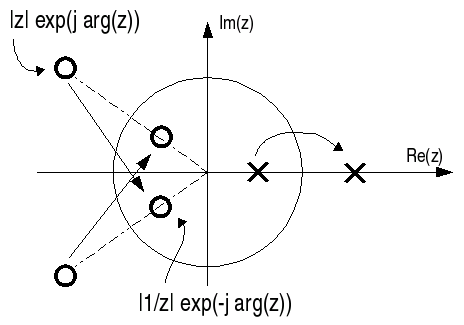
\includegraphics[height=4cm]{img/zeta05.png}\\
\end{figure}
\begin{align*}
	G_1(z) &= \frac{(z-z_1^{-1})(z-z_2)(z-z_2^*)(z-z_3^*)(z-z_3) }{poli}\\
	G_2(z) &= \frac{(z-z_1)(z-z_2^{-1})(z-(z_2^*)^{-1})(z-z_3)(z-z_3^*)}{poli}\\
	G_3(z) &= \frac{(z-z_1^{-1})(z-z_2^{-1})(z-(z_2^{-1})^*)(z-z_3)(z-z_3^*)}{poli}
\end{align*}

\subsubsection{Sistemi passa tutto}
Sistema che in cascata a un altro non cambia la risposta in modulo complessiva.\\
Se 
$$G(z)=G'(z)\cdot\frac{z^{-1}-a^*}{1-a\cdot z^{-1}}$$ 
sistema con zero in $z={a^*}^{-1}$ e polo in $z=a$, allora
$$ C(z)=C'(z)\Rightarrow |G(f)|=|G'(f)| $$
$$ \alpha = \frac{z^{-1}-a^*}{1-az^{-1}}|_{|z|=1}=\frac{\exp(-j2\pi f)-a^*}{1-a\cdot\exp(-j2\pi f)}=
	\exp(-j2\pi f)\cdot\frac{1-a^*\cdot\exp(j2\pi f)}{1-a\cdot\exp(-j2\pi f)} $$
$$ |\alpha|=\frac{|b^*|}{|b|}=1 $$
Per sistemi con risposta all'impulso reale:
$$ G{pt}=\prod_{k=1}^{M_r}\frac{z^{-1}-d_k}{1-d_kz^{-1}}\cdot\prod_{k=1}^{M_c}
	\frac{(-z^{-1}-c_k^*)(z^{-1}-c_k)}{(1-c_kz^{-1})(1-c_k^*z^{-1})} $$
\begin{itemize}
	\item il sistema passa-tutto ammette $M_r+2M_c$ poli e zeri
	\item per sistemi causali e stabili, $|d_k|,|c_k|<1$
	\item guadagno 0dB ($|G_{pt}(f)|=1$)
\end{itemize}

\subsection{Ritardo di Gruppo}
\begin{itemize}	
	\item nell'ipotesi di sistemi PT causali stabili\\
		$r<1 \Rightarrow \tau_g > 0$
	\item filtro di ordine n:\\
		${\tau_g}_{pt} = \mbox{somma di N termini positivi}\Rightarrow \mbox{sempre positivo}$\\
		la fase \'e sempre negativa
\end{itemize}

\subsection{Sistemi a fase minima}
Sistema a fase minima: sistema con zeri contenuti nel cerchio di raggio unitario.\\
Qualsiasi sistema pu\'o essere espresso come serie di un sistema a fase minima e un sistema passa-tutto.
$$ G(z)=G_{min}(z)\cdot G_{pt}(z) $$
Dato $G_{min}(z)$, il suo inverso (con risposta all'impulso $g_I[n]$ dove $g_I[n]*g[n]=\delta[n]$) \'e:
$$ G_I(z)=G_{min}^{-1}(z) $$
ovvero i poli si scambiano con gli zeri. Di conseguenza, $G_I(z)$ rimane \emph{causale e stabile}.

\subsection{Compensazione di un sistema}
Poich\'e un sistema pu\'o essere sempre visto come un sistema a fase minima in serie a un sistema passa tutto, 
e poich\'e la caratteristica fondamentale dei sistemi a fase minima \'e che possono sempre essere invertiti, si vede
che per compensare gli effetti in modulo di un sistema reale \'e sufficiente mettergli in serie l'inverso
del sistema a fase minima.
\SISTEMASERIE{$x[n]$}{$G(z)$ reale}{$y[n]$}{$G_{min}^{-1}(z)$}{$x'[n]$}
$$G(z) = G_{pt}(z)\cdot G_{min}(z)$$
\begin{align*} 
	\Rightarrow \quad |X'(f)|&=|X(f)|\\
	\arg(X'(f))&\not= \arg(X(f))
\end{align*}

\subsection{FIR a fase lineare}
$$\arg(H(f))=\beta\cdot 2\pi f\alpha$$
\begin{itemize}
	\item Tipo 1:\\
		$h[n]$ \'e a simmetria pari: $h[M-n]=h[n]$ \\
		M (ultimo campione non nullo della sequenza) \'e pari.
	\item Tipo 2:\\
		$h[n]$ \'e a simmetria pari\\
		M dispari.
	\item Tipo 3:\\
		$h[n]$ \'e a simmetria dispari, campione in $M/2$ nullo.\\
		M pari.
	\item Tipo 4:\\
		$h[n]$ \'e a simmetria dispari, campione in $M/2$ nullo.\\
		M dispari.
\end{itemize}

\begin{align*}
	h[n] &= \pm h[M-n]\\
	&\updownarrow Z\\
	H(z) &= \pm Z\{ h[M-n] \}\\
	&= \pm \sum_{n\in Z}h[M-n]\cdot z^{-n}\\
	&= \pm \sum_{n=0}^{M} h[\underbrace{M-n}_m]\cdot z^{-n}\\
	&= \pm \sum_{m=0}^{M} h[m]\cdot z^{-(M-m)}\\
	&= \pm z^{-M}\sum_{m=0}^{M} h[m]\cdot(z^{-1})^{-m}\\
	H(z)&= \pm z^{-M}\cdot H(z^{-1})
\end{align*}
Sapendo che se $h[n]\in R$, allora gli zeri di $H(z)$ devono essere reali o complessi coniugati. Di conseguenza,
per quanto visto dall'equazione precedente, in un filtro a fase lineare se esiste $z_i$ zero di $H(z)$ deve
esistere anche $z^{-1}_i$. La formula generale \'e:
$$ H(z)=\prod_{i=1}^{M_r}(z-z_i)(z-z_i^{-1})\cdot \prod_{j=1}^{M_1}(z-z'_\gamma)\cdot
	\prod_{k=1}^{M_c}(z-z''_n)(z-z^{''*}_n) \cdot$$ 
$$	\cdot\prod_{k=1}^{M}(z-z''_n)(z-z^{''*}_n)(z-z_n^{''-1})(z-(z''_n)^{-1 *})\cdot
	\prod_{l=1}^{M_{c1}}(z-z'''_l)(z-z^{'''*}_l)  $$
Con:
$$ z_i\in R\quad,\quad z'_\gamma\in\Gamma_1\cap R\quad,\quad z''_n\in C\backslash R\quad,
	\quad z'''_l \in \Gamma_1 \cap \{ C\backslash R \}$$

\subsection{Caso degli zeri in $\pm 1$}
\begin{itemize}
	\item Tipo 1:
		$h[n]$ pari, M pari\\
		(z=1) $H(1)=H(1)$ quindi z=1 \emph{pu\'o} essere uno zero\\
		(z=-1) $H(-1)=H(-1)$ quindi z=-1 \emph{pu\'o} essere uno zero
	\item Tipo 2:
		$h[n]$ pari, M dispari.\\
		(z=1) $H(1)=H(1)$ quindi z=1 \emph{pu\'o} essere uno zero\\
		(z=-1) $H(-1)=(-1)^{2k-1}H(-1)$ quindi z=-1 \emph{deve} essere uno zero
	\item Tipo 3:
		$h[n]$ dispari, M pari.\\
		(z=1) $H(1)=H(-1)$ quindi z=1 \emph{deve} essere uno zero\\
		(z=-1) $H(-1)=(-1)^{2k}H(-1)=-H(-1)$ quindi z=-1 \emph{deve} essere uno zero
	\item Tipo 4:
		$h[n]$ dispari, M dispari.\\
		(z=1) $H(1)=H(-1)$ quindi z=1 \emph{deve} essere uno zero\\
		(z=-1) $H(-1)=(-1)^{2k+1}H(-1)=H(-1)$ quindi z=-1 \emph{pu\'o} essere uno zero
\end{itemize}

\section{Discrete Fourier Transform DFT}
$$ x_a(t) \longleftrightarrow X_a(f)=\int_{-\infty}^{\infty}x_a(t)\cdot\exp(-j2\pi ft)\, dt $$
$$ x[n] \longleftrightarrow X(f)=\sum_{n=-\infty}^{\infty}x[n]\cdot \exp(-j2\pi fn)  $$
E se noi campioniamo nel dominio delle frequenze? Innanzitutto avremo una ripetizione nei tempi.\\\\
Definisco:
\begin{align*}
	X[k] &= X(f)|_{f=\frac kN}
	&\mbox{(su intervalli di lunghezza 1 avr\'o N campioni)}\\
	&=\sum_{n=-\infty}^{\infty}x[n]\cdot\exp\Bigr( -j2\pi \frac{kn}N \Bigr)
	&\mbox{(periodica di periodo N)}\\
	&= \sum_{n\in Z} x[n]\cdot W_N^{-nk}
\end{align*}
definendo $W_N$ come prima radice N-esima di 1 nei complessi (escluso 1)
$$ W_N \stackrel{\triangle}{=} \exp\Bigr( j\frac{2\pi}{N} \Bigr) $$
$k$ \'e considerato nell'intervallo:
\begin{itemize}
	\item $0,1,\dots,N-i$
	\item $-int(N/2),\dots,int(N/2)$ se N dispari, oppure\\
		$-N/2,\dots,N/2$ se N pari
\end{itemize}

\subsection{DFT inversa}
Partiamo dall'inversa della DTFT:
$$x[n] = \int_{-\frac 12}^{\frac 12}X(f)\cdot\exp(j2\pi fn)\,df\quad\forall n$$
e poi approssimiamo l'integrale come una somma di rettangolini di larghezza 1/N:
\begin{align*}
	x_p[n] &= \sum_{k=0}^{N-1}X[k]\cdot\underbrace{\exp\Bigr(-j2\pi \frac{kn}{N}\Bigr)}_{W_N^{kn}}\cdot \frac1N\\
	&= \frac1N \cdot\sum_{k=0}^{N-1}\Bigr( \sum_{l\in Z} x[l]\cdot W_N^{-lk} \Bigr)\cdot W_N^{nk}\\
	&= \frac1N \cdot\sum_{l\in Z}x[l]\cdot \sum_{k=0}^{N-1}W_N^{(n-l)k}\\
	&= \sum_{l\in Z}x[l]\cdot \Bigr( \underbrace{\frac1N \sum_{k=0}^{N-1}W_N^{(n-l)k}}_
		{=1 \mbox{ se } n-l=mN \mbox{ , 0 altrimenti}} \Bigr)\\
	&= \sum_{m\in Z}x[n+mN]
\end{align*}
Come si vede. il campionamento ha portato alla creazione di repliche di $x[n]$ con passo N.\\
\\
Il passaggio sopra si spiega come:
$$ \sum_{k=0}^{N-1}(W_N^m)^k=\frac{1-(W_N^m)^N}{1-W_N^m} \qquad \mbox{serie geometrica}$$
che vale zero in tutti i casi tranne quando $m=kN$\\
\\
Esiste dunque la possibilit\'a di aliasing temporale, che si pu\'o evitare:
\begin{itemize}
	\item Quando $x[n]$ \'e a durata finita M, scegliendo $N \geq N$
	\item Quando $x[n]$ \'e periodico di periodo M, scegliendo $N=M$
\end{itemize}

\subsection{Formule per le serie a durata finita}
\begin{align*}
	\DFT_N(x[n]) &\stackrel{\triangle}{=}X[k]=\sum_{n=n_0}^{n_0+N-1}x[n]\cdot W_N^{-nk} &k=0,1,\dots,N-1\\
	\DFT^{-1}(X[k]) &\stackrel{\triangle}{=}x[n]=\frac1N \sum_{k=0}^{N-1}X[k]\cdot W_N^{nk}&n=n_0,\dots,n_0+N-1
\end{align*}

\begin{equation*}
	\begin{pmatrix}
		X[0] \cr X[1] \cr \vdots \cr X[N-1]
	\end{pmatrix}
	=
	\underbrace{
	\begin{pmatrix}
		1 & \dots & \dots & \dots & 1 \cr
		1 & W_N^{-1} & \dots &\dots & W_N^{-(N-1)} \cr
		\vdots & \vdots & \vdots & \ddots & \vdots \cr
		1 & W_N^{-(N-1)} & W_N^{-2(N-1)} & \dots & W_N^{-(N-1)^2}
	\end{pmatrix}
	}_{\mbox{matrice W}}
	\cdot
	\begin{pmatrix}
		x[0] \cr x[1] \cr \vdots \cr x[N-1]
	\end{pmatrix}
\end{equation*}
La DFT pu\'o essere vista come una semplice operazione matriciale.

\subsection{Propriet\'a di $W_N$}
$$W_N \stackrel{\triangle}{=} \exp\Bigr( \frac{j2\pi}N \Bigr)$$
\begin{enumerate}
	\item Espandibilit\'a\\
		$$ W_N^{k+l}=W_N^k\cdot W_N^l $$
	\item Periodicit\'a di N
		$$ W_N^{k+lN}=W_N^{k} \qquad W_N^k = W_N^{(k\, mod\, N)} $$
	\item 
		$$ W_N^{lN}=1\qquad W_N^{N/2}=W_N^{N/2+lN}=-1 \qquad W_N^{N/2+l}=-W_N^l \qquad W^2_N = W_{N/2} $$
	\item Ortonormalit\'a
		\begin{align*}
			\frac1N \cdot \sum_{n=0}^{N-1}W_N^{kn}&= 1 \quad k=ln\\
			&= 0 \quad \mbox{altrimenti}
		\end{align*}
\end{enumerate}

Esempio: N=5
\begin{figure}[h] %  figure placement: here, top, bottom, or page
   \centering
   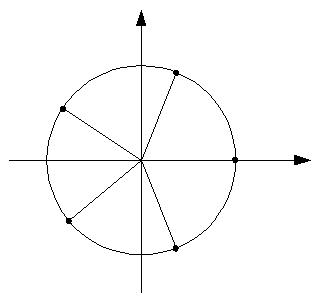
\includegraphics[width=2in]{img/wn5.jpg} 
\end{figure}
\begin{align*}
	&\sum_{k=0}^{4}\Bigr[ \exp\Bigr( j2\pi\frac k5 \Bigr) \Bigr]^0=5\\
	&\sum_{k=0}^{4}\Bigr[ \exp\Bigr( j2\pi\frac k5 \Bigr) \Bigr]^1=0\\
	&\sum_{k=0}^{4}\Bigr[ \exp\Bigr( j2\pi\frac k5 \Bigr) \Bigr]^{2-3-4}=0&\mbox{i vettori si scambiano tra di loro}\\
	&\sum_{k=0}^{4}\Bigr[ \exp\Bigr( j2\pi\frac k5 \Bigr) \Bigr]^5=5&\mbox{i vettori si spostano tutti in 1}\\
\end{align*}

Conseguenza delle propriet\'a viste \'e che la matrice W(NxN) \'e composta solo da N elementi diversi.

\newpage

\subsection{Complessit\'a calcolo DFT}
A prima vista il calcolo della DFT richiede $(N^2 moltiplicazioni + N(N-1) addizioni complesse)$, mentre
in realt\'a con algoritmi veloci che sfruttano la struttura della matrice W la complessit\'a varia da
$O(N)$ a $O(\frac N2 \log_2 N)$ operazioni complesse.

\begin{figure}[htbp] %  figure placement: here, top, bottom, or page
   \centering
   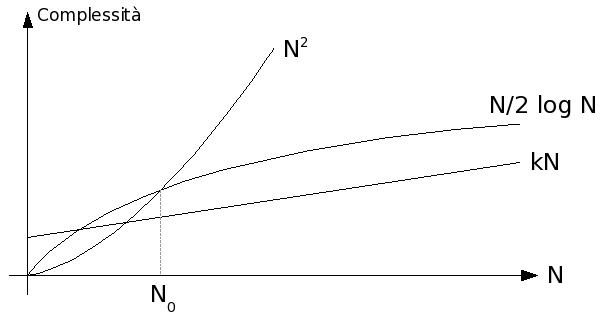
\includegraphics[width=3in]{img/compless.jpg} 
\end{figure}

\subsection{DFT e trasformata Z}
$$ X(z)=\frac{z^{-N}-1}{N}\cdot\sum_{k=-\frac N2}^{\frac N2-1}x[k]\cdot\frac{1}{W_N^k\cdot z^{-1}-1} $$
Dimostrazione:
\begin{align*}
	X(z) &= \sum_{n=0}^{N-1}x[n]\cdot z^{-n} &ROC\{ z:|z|>0 \} \mbox{ per seq. causali di durata N}\\
	&= \sum_{n=0}^{N-1}\Bigr[ \frac 1N \cdot \sum_{k=-\frac N2}^{\frac N2-1} x[k]\cdot W_N^{nk} \Bigr]\cdot z^{-n}\\
	&= \frac1N \cdot \sum_{k=-\frac N2}^{\frac N2-1}x[k]\cdot \sum_{k=0}^{N-1}(W_N^k\cdot z^{-1})^n\\
	&= \frac1N \sum_{k=-\frac N2}^{\frac N2-1}x[k]\cdot\frac{\overbrace{W_N^{kN}}^{1}\cdot z^{-N} -1}{W_N^K\cdot z^{-1}-1}&CVD
\end{align*}

\subsection{DFT e DTFT}
$$ X(f)=\frac1N \cdot \sum_{k=-\frac N2}^{\frac N2-1}x[k]\cdot \frac{\sin(\pi fN)}
	{\sin\Bigr( \pi\Bigr( f-\frac KN \Bigr) \Bigr)}\cdot\exp\Bigr(j\pi\Bigr(f\Bigr(1-N\Bigr)\frac KN\Bigr)\Bigr) $$
\\
\\
\\
{\huge Manca lezione luned\'i 13-03-2006}
\\
\\
\subsection{Propriet\'a DFT}

\subsubsection{Interpolazione numerica della DFT}
\begin{align*}
	x'[n] &= x[n]& n=0,1,\dots,N-1\\
	&= 0 & n=N,\dots,2N+1\\
	X'(f)&=X(f)
\end{align*}
\begin{align*}
	X'[h] =& \sum_{n=0}^{N-1}x[n]\cdot W_{2N}^{-hn} &(=\DFT_{2N}(x[n]))\\\\
	=& X[l] &k=2l\\
	&X(f)|_{f=\frac K{2N}} &k=2l+1
\end{align*}
Aggiungendo N zeri si \'e interpolato esattamente i valori di $X(f)$ in $k=\frac{2l+1}{2N}$

\subsubsection{Calcolo della DFT di un segnale periodico su 2 periodi}
\begin{align*}
	X[h] &= \sum_{n=0}^{2N-1}x[n]\cdot W_{2N}^{-nh}\\
	&= \sum_{n=0}^{N-1}x[n]\cdot W_{2N}^{-nh} +\sum_{n=N}^{2N-1}x[n]\cdot W_{2N}^{-nh}\\
	&= \sum_{n=0}^{N-1}x[n]\cdot W_{2N}^{-nh} + \sum_{n=0}^{N-1}x[n-N]\cdot W_{2N}^{-(n-N)h}\\
	&= \sum_{n=0}^{N-1}x[n]\cdot \underbrace{\Bigr( W_{2N}^{-nh}+W_{2N}^{-(n-N)h} \Bigr)}_
		{= 2W_{2N}\mbox{ se }h=2l\mbox{ , 0 altrimenti}}\\\\
	&= 2\cdot y\Bigr( \frac hN \Bigr) &\mbox{per h pari}\\
	&= 0& \mbox{per h dispari}
\end{align*}
Con 
$ y[n] = \sum_{n=0}^{N-1}x[n]\cdot W_{N}^{-nh} $\\\\

Esempio:\\
\begin{figure}[h] %  figure placement: here, top, bottom, or page
   \centering
   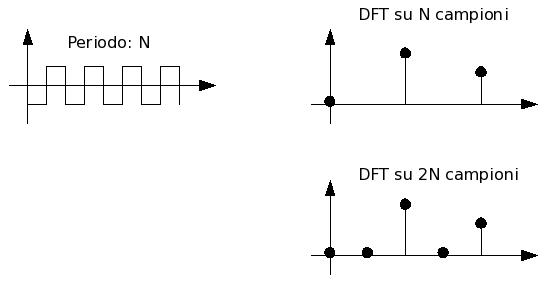
\includegraphics[width=4in]{img/dft2periodi.jpg} 
\end{figure}

Quindi i valori su un periodo del segnale di partenza sono pi\'u che sufficienti per calcolare la DFT (sempre
che il segnale sia perfettamente periodico, ovviamente).

\subsection{Convoluzione indiretta}

\subsubsection{Segnali a durata limitata}
$x[n]$ segnale di durata $N_x$ (primo campione non nullo in 0)\\
$y[n]$ segnale di durata $N_y$ (primo campione non nullo in 0)\\
\\
\begin{align*}
	x'[n] &= x[n] &n=0,\dots,N_x-1\\
	&= 0 &n=N_x,\dots,\underbrace{N_x+N_y-1}_{=N-1}\\
	y'[n] &= y[n] &n=0,\dots,N_y-1\\
	&= 0 &n=N_y,\dots,N_x+N_y-1
\end{align*}
Calcolo le DTF, ottengo $X'[k]$ e $Y'[k]$
$$Z[k]=X[k]\cdot Y[k] \stackrel{\DFT_N^{-1}}{\longrightarrow}z[n]=x[n]*y[n]$$

\subsubsection{Segnali dello stesso periodo N}
$$ x_p[n] \stackrel{\DFT}{\longrightarrow}X_p[k] $$
$$ y_p[n] \stackrel{\DFT}{\longrightarrow}Y_p[k] $$
$$ Z_p[k]=\frac1N\cdot X_p[k]\cdot Y_p[k] \longrightarrow z_p[n]=x_p[n]\convcirc y_p[n] $$

\subsubsection{Segnali di periodi diversi $N_x$, $N_y$}
$$ z_p[n]=\frac1N \sum_{m=n_0}^{n_0+N-1}x_p[n]\cdot y_p[n-m]\quad \mbox{con } N=MCM(N_x,N_y) $$
Esempio:\\\\
Supponiamo $N_x=12$ e $N_y=10$, quindi il loro $MCM=60$.\\
Quindi facciamo la DFT di $x$ e $y$ su 60 campioni, ovvero rispettivamente 5 e 6 periodi.
Si aggiungono quindi 4 campioni nulli tra ciascun campione di $X[k]$ e 5 campioni nulli tra i campioni di $Y[k]$.\\\\
Come si vede, c'\'e "battimento" tra valori di $X[k]$ e $Y[k]$ solo per un campione, ovvero $X[30]\cdot Y[30]$\\
(pi\'u in generale, per valori di $k$ pari a $N/mcd(N_x,N_y)$ e multipli).\\\\
$z_p[n]$ ha periodo pari a $mcd(N_x,N_y)$ e vi sono $mcm(N_x,N_y)/mcd(N_x,N_y)$ periodi osservati generati se
$X[k]$ e $Y[k]$ sono calcolati su $N=mcm(N_x,N_y)$.

\newpage

\subsection{Convoluzione lineare di sequenze lunghe}
Nel caso di sequenze in ingresso molto lunghe (tipo 1000 o pi\'u campioni) e filtri con risposta all'impulso anch'essa
lunga (anche qui, tipo 1000 campioni), risulta computazionalmente pressoch\'e impossibile realizzare la convoluzione
indiretta come visto in precedenza, poich\'e sarebbe necessario trasformare due sequenze molto lunghe, moltiplicarle e
estrarne l'antitrasformata.\\
Esistono dei metodi per dividere questo procedimento in passi di complessit\'a accettabile.

\subsubsection{Overlap-add}
Divido $x[n]$ in K sequenze contigue di lunghezza M.
\begin{align*}
	x[n]=\sum_{k=0}^{K} x_k[n] \qquad x_k[n] &= x[n+kM] &n=0,1,dots,M-1\\
	&=0 &\mbox{altrove}
\end{align*}
$$ y[n] = \Bigr( \sum_{k=0}^{M}x_k[n] \Bigr)*h[n] = \sum_{k=0}^{M}\Bigr( \underbrace{x_k[n]*y[n]}
	_{\mbox{(in maniera indiretta)}}
\Bigr) $$

\begin{figure}[h] %  figure placement: here, top, bottom, or page
   \centering
   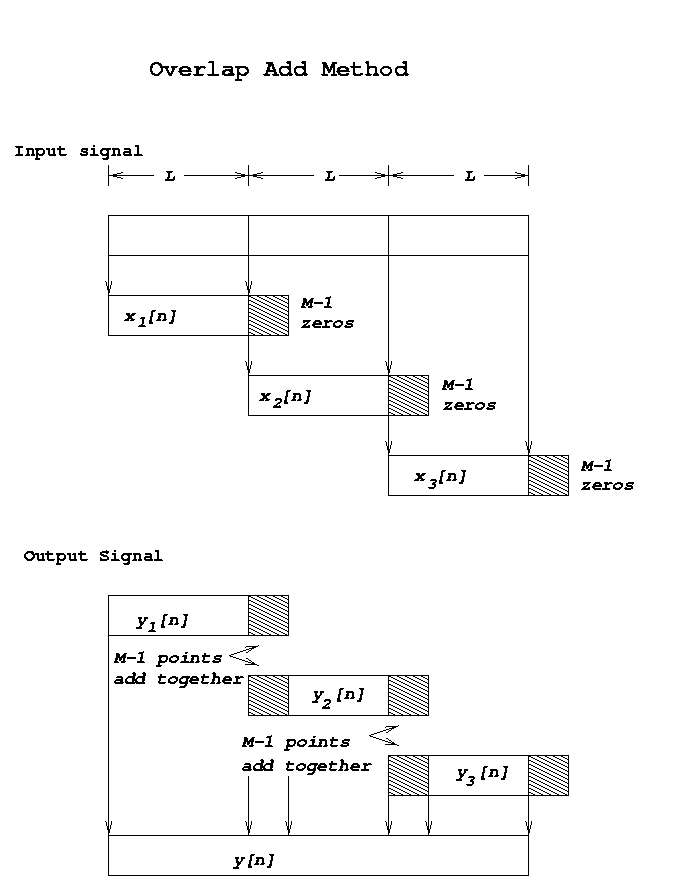
\includegraphics[width=7cm]{img/overlap_add.jpg} 
\end{figure}

$y[n]$ si ottiene mantenendo i valori delle $y_k[n]$ esclusi gli $N_h-1$ valori di ciascuna sezione filtrata che
vanno sommati agli $N_h-1$ valori iniziali delle sezioni filtrate successive.\\
\\
Esempio:\\
$N_h=1000$, $M=1000$, $\Rightarrow$ $y_k[n]=x_k[n]*h[n]$ sequenze lunghe 1999 campioni (portati alla prima potenza
di 2 disponibile, ovvero 2048).\\
Per ogni sezione, la complessit\'a di calcolo \'e:
$$O\Bigr( \frac{2048}{2}\cdot \log_2 2048 \Bigr) \approx 11264 \mbox{ operazioni}$$
Mentre con il metodo diretto avremmo avuto, per ciascuna operazione:
$$1000^2=10^6 \mbox{ operazioni}$$

\subsubsection{Overlap-save}
Scompongo $x[n]$ in K sezioni di durata M sovrapposte di $N_h-1$ campioni, designate $x_k'[n]$ (ovviamente diverse
dalle $x_k[n]$ del caso precedente!). Supponendo:
\begin{align*}
	h'[n]&=h[n]&n=0,1,\dots,N_h-1\\
	&=0 &n=N_h,\dots,M-1
\end{align*}
Abbiamo che:
\begin{align*}
	x'_l[n] &\stackrel{\DFT_M}{\longrightarrow} X'_l[k]\\
	h'[n] &\stackrel{\DFT_M}{\longrightarrow} H'[k]\\
\end{align*}
$$ Y'_l[k]=X'_l[k]\cdot H'[k] \stackrel{\DFT^{-1}_M}{\longrightarrow} y'_l[n] $$
Gli $N_h-1$ primi campioni di $y'_l[n]$ sono affetti da aliasing temporale a causa della convoluzione circolare vista 
dalla DFT. Vanno dunque scartati, mentre gli altri possono essere direttamente \emph{mantenuti} in quanto corretti.

\begin{figure}[h] %  figure placement: here, top, bottom, or page
   \centering
   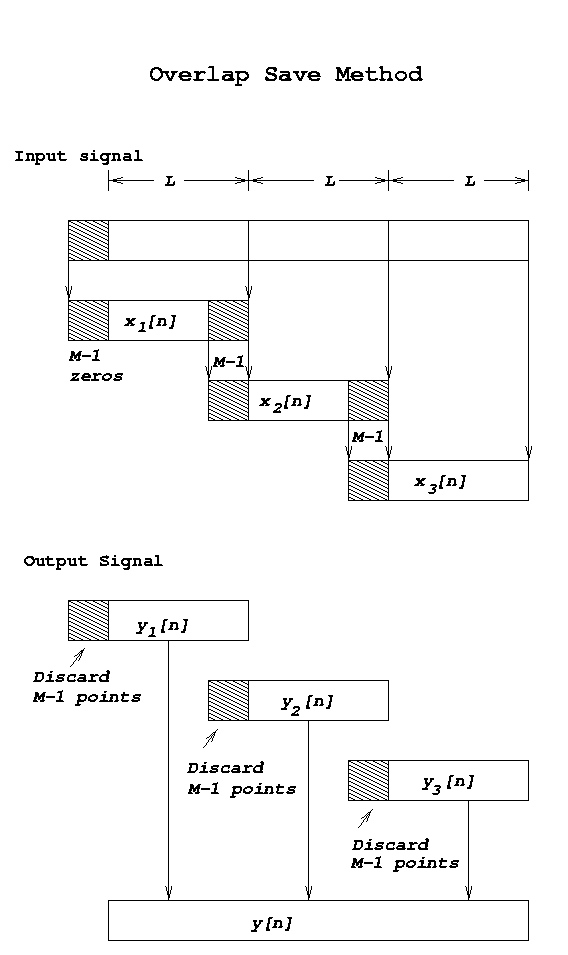
\includegraphics[width=7cm]{img/overlap_save.jpg} 
\end{figure}

\newpage

\section{Analisi Spettrale}
Stima con DFT di $X(f)$ per $x[n]$ non periodica lunga.\\
Ipotesi su $W_N[n]$:
\begin{itemize}
	\item lunga $N+1$
	\item simmetria pari
	\item centrata in 0
	\item $W_N[0]=1=\int_{u}^{u+1}W_N(f)\,df$
\end{itemize}
\begin{align*}
	x_N[n] &= x[n]\cdot W_N[n] \quad \mbox{(finestra di misura di }x[n]\mbox{)}\\
	&\downarrow \DTFT\\
	X_N(f) &= \int_u^{u+1}X(g)\cdot W_N(f\cdot g)\,dg=W_N(f)\convcirc_1 X(f)
\end{align*}
$$W_N(f)=\sum_{n=-N/2}^{N/2} W_N[n]\cdot \exp(-j2\pi fn)$$

\newpage

\subsection{Finestra Rettangolare}
$$ W_N[n] \longrightarrow r_N[n]=\mbox{rect}_N[ n+N' ] \qquad N'=\mbox{int}\Bigr( \frac{N}{2} \Bigr)$$
$$ R_N(f)=\frac{\sin(\pi fn)}{\sin(\pi f)} $$
$$ |R_N(f)| \mbox{ massimo }\approx \frac{2K+1}{2N} $$
$$\alpha_N = |\frac{R_N(0)}{R_N(3/2N)}|\approx 4,5\qquad (N<100)$$
$$\lim_{N\to\infty}\alpha_N = \frac{3\pi}2\approx 4,712$$
Che succede?\\
Supponendo in ingresso una sinusoide (in frequenza, un impulso in $f_0$), ho, moltiplicando per la finestra 
(quindi convolvendo in frequenza con $R_N(f)$) ottengo:
\begin{figure}[h] %  figure placement: here, top, bottom, or page
   \centering
   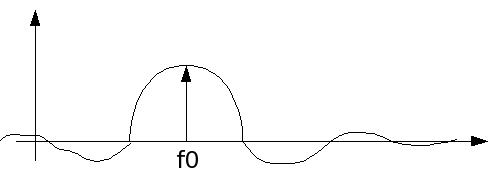
\includegraphics[width=5cm]{img/rettangolare1.jpg} 
\end{figure}

Si notano due cose:
\begin{enumerate}
	\item qualunque sia il valore di N, comunque il valore di $\alpha_N$ non cambia, e questo porta 
		ad avere nello spettro finestrato dei picchi al di fuori della frequenza $f_0$.
	\item N influenza invece la frequenza delle oscillazioni, quindi la risoluzione frequenziale. Infatti,
		con N elevato il "sinc" corrispondente esaurisce in suo lobo principale molto in fretta, 
		non andando a influenzare quindi i "sinc" corrispondenti ad eventuali altre frequenze presenti.
\end{enumerate}

\begin{figure}[h] %  figure placement: here, top, bottom, or page
   \centering
   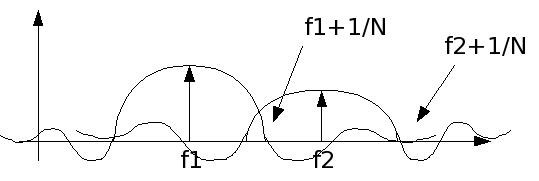
\includegraphics[width=2in]{img/rettangolare2.jpg} 
   \caption{N piccolo}
   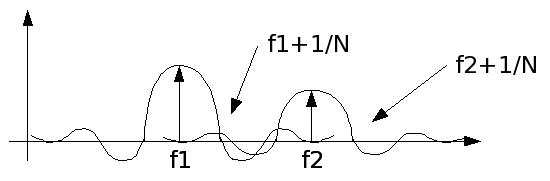
\includegraphics[width=2in]{img/rettangolare3.jpg} 
   \caption{N grande}
\end{figure}

$\Delta_R$: lunghezza del lobo principale $=\frac2N$\\
determina la capacit\'a di risoluzione frequenziale dell'analisi mediante finestramento.\\
\\
Si converte $\alpha$ (rapporto tra il max del lobo principale e il max del secondo lobo di $W_N(f)$ in modulo) in
$\lambda$, che ne \'e una misura in dB.
$$ \lambda_R^{(N)} =-20\cdot\log_{10}|\frac{R_N(0)}{R_N(f_0)}|=-13\,dB \qquad f_0\mbox{ posizione del max del 
	secondo lobo}$$

\subsection{Finestra Triangolare}

%fine teoria -------------------------------------------------------------------------------------------------
%\end{document}

\clearpage
\appendix

\section{Esempi}

\subsection{Parte pari e parte dispari (per sequenze causali)}

\begin{figure}[htbp] %  figure placement: here, top, bottom, or page
   \centering
   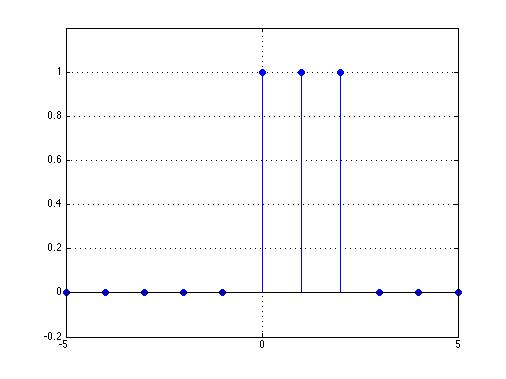
\includegraphics[height=3.5cm]{img/rect-tutteparti.jpg} 
   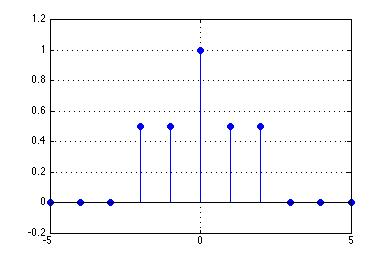
\includegraphics[height=3.5cm]{img/rect-partepari.jpg}
    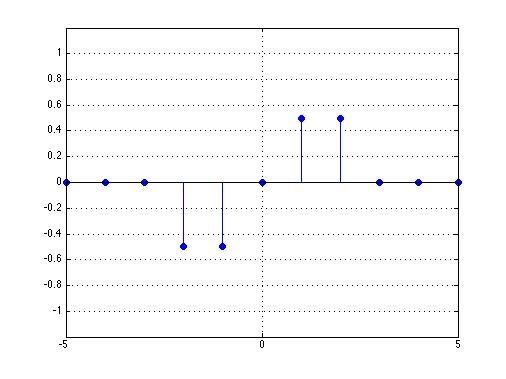
\includegraphics[height=3.5cm]{img/rect-partedispari.jpg}
    \caption{Segnale di partenza, parte pari, parte dispari}
\end{figure}
\begin{align*}
	x_p[n] &= \frac12 x[n]&\mbox{per }n>0\\
		&= x[0]&\mbox{per }n=0\\
	x_d[n] &= \frac12x[n]&\mbox{per } n>0\\
		&= 0&\mbox{per } n=0
\end{align*}

\subsection{Calcolo di energie e potenze di segnali}

\paragraph{Esempio 1}
$$x[n]=2\mbox{rect}_2[n]+\mbox{rect}_2[n-2]+i(\delta[n]-\delta[n-3])$$
\begin{figure}[htbp] %  figure placement: here, top, bottom, or page
   \centering
   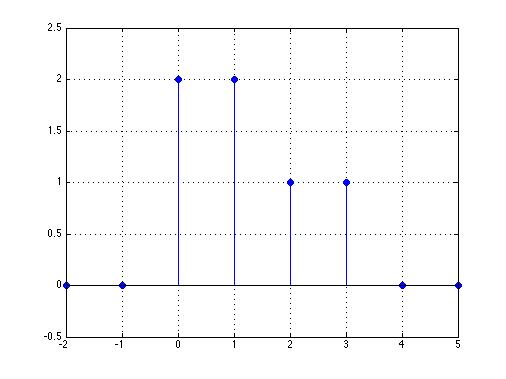
\includegraphics[width=2in]{img/es04-01.jpg} 
   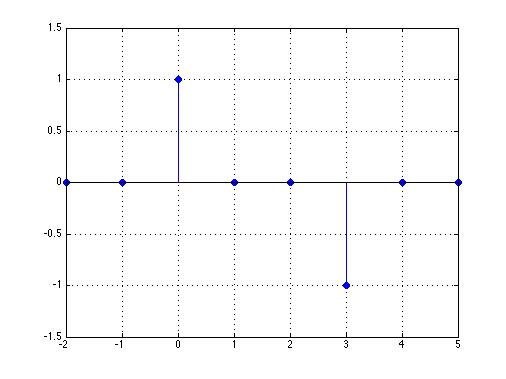
\includegraphics[width=2in]{img/es04-02.jpg} 
   \caption{Parte reale e parte immaginaria del segnale}
\end{figure}
$$W_x=\sum_{n=-\infty}^{+\infty}|x[n]|^2=|2+i|^2+2^2+1^2+|1-i|^2=12$$

\paragraph{Esempio 2}
$$x[n]=2\sum_{k=0}^\infty(-1)^k\delta[n-k]$$
\begin{align*}
	P_x&=\lim_{N\to\infty}\frac1{2N+1}\sum_{n=-N}^{N}|x[n]|^2\\
		&=\lim_{N\to\infty}\frac1{2N+1}\sum_{n=0}^{N}2^2\\
		&=\lim_{N\to\infty}\frac1{2N+1}4(N+1)=2  
\end{align*}

\subsection{Convoluzione lineare}

\paragraph{Esempio 1}
$$x_1[n]=a^n\cdot\varepsilon[n]$$ $$x_2[n]=\mbox{rect}_N[n]$$
\begin{align*}
x_1[n]*x_2[n] &= \sum_{m=0}^{n}x_1[n]\cdot\mbox{rect}_N[n-m]\\
	&= \sum_{m=0}^{n}\cdot a^m=\frac{1-a^{n+1}}{1-a}&\mbox{per }0\leq n\leq N\\
x_1[n]*x_2[n] &= \sum_{m=n-N+1}^{n}a^m\cdot 1=\\
	&\downarrow m'=m-(n-N+1)\\
	&= \sum_{m'=0}^{N-1}a^{m'+(n-N+1)}\\
	&= a^{n-N+1}\cdot\sum_{m'=0}^{N-1}a^{m'}=a^{n-N+1}\frac{1-a^N}{1-A}&\mbox{per }n\geq N
\end{align*}

\paragraph{Esempio grafico 1}
$$ z[n] = x[n]*y[n] = \sum_{n=-\infty}^{\infty} x[m]\cdot y[n-m]$$
\begin{align*}
	x[n]&=\mbox{rect}_4[n]\\
	y[n]&=2\mbox{rect}_3[n]
\end{align*}
\begin{center}
	\begin{tabular}{cc}
		\includegraphics[height=2.5cm]{img/es01a.png}
		&
		\includegraphics[height=2.5cm]{img/es01b.png}
	\end{tabular}\\
	\includegraphics[height=3cm]{img/es01c.png}
\end{center}

\paragraph{Esempio grafico 2}
\begin{align*}
	x[n]&=\alpha^n\cdot\varepsilon[n]\\
	y[n]&=\beta^n\cdot\varepsilon[n]&\mbox{con }\mid\alpha\mid,\mid\beta\mid < 1
\end{align*}
\begin{center}
	\includegraphics[height=2.5cm]{img/es02a.png}
\end{center}
Si pu\'o risolvere solo per via analitica:
\begin{align*}
	x[n]*y[n] &= \sum_{m=0}^{n}x[m]y[n-m]\\
	&= \sum_{m=0}^{n}\alpha^m\cdot \beta^{n-m}\\
	&= \beta^n\sum_{m=0}^{n}\Bigr( \frac{\alpha}{\beta} \Bigr)^m&\mbox{serie geometrica}\\
	&=\beta^n\cdot\frac{1-\Bigr( \frac{\alpha}{\beta} \Bigr)^{n+1}}{1- \frac{\alpha}{\beta}}
\end{align*}

\subsection{Convoluzione circolare}

\subsubsection{Esempio}
Prendiamo $x[n]$ periodico di periodo $M_x$ e $y[n]$ periodico di periodo $M_y$.
$$ x[n] \otimes_M y[n] = \sum_{m=n_0}^{n_0+M-1}x[m]y[n-m] $$
con $n_0$ qualsiasi e $M=mcm(M_x,M_y)$. Ad esempio:\\
\begin{center}
	\includegraphics[height=2.5cm]{img/es03a.png}\\
	\includegraphics[height=2.5cm]{img/es03b.png}
\end{center}
Per svolgere la convoluzione circolare devo eseguire i seguenti passi:
\begin{itemize}
	\item cambio gli indici (n $\rightarrow$ m)
	\item ribalto $y[m]$ rispetto a un punto qualsiasi\\
		\includegraphics[height=2cm]{img/es03c.png}
	\item traslo $y[m]$ di $n$\\
		\includegraphics[height=2cm]{img/es03d.png}
	\item lo moltiplico per $x[m]$\\
		\includegraphics[height=2.5cm]{img/es03e.png}
	\item sommo gli elementi e ottengo il valore di $z[n]$ con l'$n$ scelto.
	$$ z[1]=2+4+6+2=14 $$
	\item ripeto per tutti gli $n$.
\end{itemize}

\subsection{Generazione di sequenze casuali}

\subsubsection{Sequenze con PDF arbitraria}
A partire da una sequenza X (variabile casuale) con distribuzione uniforme su $[0,1]$ � possibile ricavare una sequenza Y con distribuzione scelta. In questo esempio vogliamo ottenere:
$$f_Y(y)=\frac1A \mbox{tri}\Bigr( \frac yA \Bigr)$$
Soluzione: per prima cosa bisogna scrivere la formula della distribuzione $f_Y(y)$:
\begin{align*}
	f_Y(y) &= -\frac1{A^2}y+\frac1A &y\geq0\\
		&= \frac1{A^2}y+\frac1A&y>0
\end{align*}
Poi si integra per trovare $F_Y(y)$:
\begin{align*}
	F_Y(y) &= 0&y<-A\\
		&= \int_{-A}^{y}\Bigr(\frac1A+\frac z{A^2}\Bigr)dz= \\
		&= \Bigr(\frac y{\sqrt2A}+\frac1{\sqrt 2} \Bigr)^2&-A<y<0\\
		&=  \int_{-A}^{0}\Bigr(\frac1A+\frac z{A^2}\Bigr)dz+\int_{0}^{y}\Bigr(-\frac z{A^2}+\frac1A\Bigr)=\\
		&= 1-\Bigr( \frac y{\sqrt 2 A}-\frac1{\sqrt2}\Bigr)^2&0<y<A\\
		&= 1&y>A
\end{align*}

E poi si calcola $F^-1_Y(y)$:
\begin{itemize}
	\item Dove $-A\leq y<0$ (quindi $0\leq x<\frac12$):
		\begin{align*}
			x&=\Bigr(\frac y{\sqrt2 A}+\frac1{\sqrt2}\Bigr)^2\\
			\sqrt x &= \frac y{\sqrt2 A}+\frac1{\sqrt2}\\
			y&= \sqrt{2x}A-A
		\end{align*}
		
	\item Dove $0<y<A$ (quindi $\frac12\leq x<1$):
		$$y=-\sqrt{2(1-x)}A+A$$
\end{itemize}

A questo punto � sufficiente moltiplicare ciascun elemento della sequenza uniforme per $F^{-1}_Y(y)$ per ottenere una sequenza con dstribuzione triangolare.
\begin{figure}[htbp] %  figure placement: here, top, bottom, or page
   \centering
   \includegraphics[width=12cm]{img/cambiopduniftri.jpg} 
   \caption{Istogrammi di $X$ e $Y$}
\end{figure}

%fine esercitazione -------------------------------------------------------------------------------------------------
\clearpage
\section{Matlab}

\subsection{Segnali e Operazioni Elementari}

\subsubsection{Funzioni per generare segnali elementari}

\paragraph{Rettangolo}
\input{script/rect}

\begin{itemize}
	\item Delta di Dirac
		\begin{verbatim}
function x = delta(tempo)
%TEMPO base dei tempi
x = zeros(1, length(tempo));
for i=1:length(tempo)
    if (tempo(i) == 0) 
        x(i) = 1;
    else
        x(i) = 0;
    end
end
		\end{verbatim}
	
	\item Gradino
		\begin{verbatim}
function x = epsilon(tempo)
%TEMPO base dei tempi
x = zeros(1, length(tempo));
for i=1:length(tempo)
    if (tempo(i) >= 0) 
        x(i) = 1;
    else
        x(i) = 0;
    end
end
		\end{verbatim}

	\item Rettangolo
		\begin{verbatim}
function x = rect(tempo, numcampioni)
%TEMPO base dei tempi
%NUMCAMPIONI numero di campioni che compongono il rettangolo
x = zeros(1, length(tempo));
for i=1:length(tempo)
    if (tempo(i) >= 0 && tempo(i) < numcampioni) 
        x(i) = 1;
    else
        x(i) = 0;
    end
end
		\end{verbatim}

\end{itemize}

\subsubsection{Operazioni elementari}

\begin{itemize}
	\item Traslazione di un segnale
		\begin{verbatim}
function x = trasla(segnale, quantita)
%TEMPO base dei tempi
%QUANTITA fattore di traslazione
x = zeros(1, length(segnale));
for i=1:length(segnale)
    if (i-quantita <= length(segnale) && i-quantita > 0)
        x(i) = segnale(i-quantita);
    else
        x(i) = 0;
    end
end
		\end{verbatim}
		
	\item Ribaltamento di un segnale rispetto all'origine dell'asse dei tempi
		\begin{verbatim}
function x = ribalta(tempo,segnale)
%TEMPO asse dei tempi
%SEGNALE il segnale da ribaltare
x = zeros(1, length(segnale));
for i=1:length(segnale)
    if (find(tempo == -tempo(i)))
        x(i) = segnale(find(tempo == -tempo(i)));
    end
end
		\end{verbatim}
		
	\item Decimazione di un segnale
		\begin{verbatim}
function x = decima(tempo, segnale, fattore)
%TEMPO base dei tempi
%SEGNALE il segnale da decimare
%FATTORE fattore di decimazione
x=zeros(1,length(tempo))
for (i=1:length(segnale))
    if (mod(tempo(i),fattore) == 0)
        x(find(tempo == (tempo(i)./fattore))) = segnale(i);
    end
end
		\end{verbatim}
		
	\item Interpolazione di un segnale
		\begin{verbatim}
function x = interpola(tempo, segnale, fattore)
%TEMPO base dei tempi
%SEGNALE il segnale da interpolare
%FATTORE fattore di interpolazione
x=zeros(1,length(tempo))
for (i=1:length(segnale))
    if (find(tempo==tempo(i)*fattore) > 0)
        x(find(tempo==tempo(i)*fattore)) = segnale(i);
    end
end
		\end{verbatim}
	
\end{itemize}


%fine documento
\end{document}
